%\documentclass[12pt]{article}
\input{/Users/joshyv/Research/misc/latex_paper.tex} 
%\newcommand{\hC}{\widehat{C}}
%\newcommand{\hn}{\widehat{n}}
\newcommand{\zzz}{z}
\newcommand{\xT}{\ve{C}}
\newcommand{\yT}{\ve{y}}
\newcommand{\nT}{\ve{n}}
\newcommand{\zT}{\ve{n}}
\newcommand{\FT}{\ve{F}}
\newcommand{\lT}{\ve{\lam}}
\newcommand{\wX}{\widehat{\ve{C}}}
\newcommand{\wY}{\widehat{\ve{Y}}}
\newcommand{\CaT}{\Cav}
\newcommand{\ax}{\argmax_{\ve{C}_t \geq 0 \forall t}}
\newcommand{\an}{\argmin_{n_t \geq 0 \forall t}}
\newcommand{\az}{\argmin_{\bM \bC \geq \ve{0}}}
\newcommand{\ath}{\argmax_{\bth \in \ve{\Theta}}}
\newcommand{\ann}{\argmin_{n_t \in \mathbb{N}_0 \forall t}}
\newcommand{\hnm}{\widehat{\bn}}
\newcommand{\hCm}{\widehat{\bC}}
\newcommand{\transpo}[1]{{#1}^{\ensuremath{\mathsf{T}}}}           % transpose
\newcommand\transp{{\!\scriptscriptstyle\mathrm T}}
%\newcommand{\hbm}{\widehat{\ve{\nu}}}
%\newcommand{\hbn}{\widehat{\bn}}
%\newcommand{\hbC}{\widehat{\bC}}

\lhead{Vogelstein JT, et al}
\rhead{Fast spike train inference from calcium imaging}
%\headheight=14.5pt

\title{Fast spike train inference from calcium imaging}

\author{Joshua T.~Vogelstein, others, Liam Paninski}

\begin{document}

\maketitle

\begin{abstract}
\begin{abstract}
Calcium imaging technologies for observing spiking activity simultaneously from large populations of neurons are quickly gaining popularity.  While the raw data are fluorescence movies, often, the underlying spike trains are of interest.  We develop here an online non-negative deconvolution filter to infer the approximately mostly likely spike trains for each neuron, given the fluorescence observations.  This algorithm outperforms optimal linear deconvolution (aka, Wiener filter) on both simulated and in vitro data, and requires approximately the same computational time.  The performance gains come from restricting the inferred spike trains to be positive (using an interior-point method), unlike the Wiener filter.  The algorithm is fast enough that even when simultaneously imaging $\approx 100$ neurons, inference can simultaneously be performed on all observed traces faster than real time.  We demonstrate that performing optimal spatial filtering on the images further refines the estimates.  Importantly, all the parameters required to perform our inference can be estimated using only the fluorescence data, obviating the need to perform simultaneous electrophysiological calibration experiments.
%A fundamental desideratum in neuroscience is to simultaneously observe the spike trains from large populations of neurons. Calcium imaging technologies are bringing the field ever closer to achieving this goal, both in vitro and in vivo. To get the most information out of these preparations, one can increase the frame rate and image field, leading to corresponding increases in temporal resolution and number of observable cells.  However, these increases come at the cost of reducing the dwell time per pixel, causing a decrease in the signal-to-noise ratio.  Thus, to maximize the utility of these technologies, powerful computational tools must be built to compliment the experimental tools.  In particular, by considering the statistics of the data --- e.g., spikes are positive --- we develop an approximately optimal algorithm for inferring spike trains from fluorescence data. More specifically, we use an interior-point method to perform a fast non-negative deconvolution, inferring the approximately most likely spike train for each neuron, given their fluorescence signals. We demonstrate using simulations and in vitro data-sets the improvement of our algorithm over optimal linear deconvolution.  Moreover, because our inference is very fast --- requiring only about 1 second of computational time on laptop to analyze a calcium trace from 50,000 image frames --- we call this approach the \foopsi filter. We demonstrate that performing optimal spatial filtering on the images further refines the estimates.  Importantly, all the parameters required to perform our inference can be estimated using only the fluorescence data, obviating the need to perform simultaneous electrophysiological experiments.  Finally, all the code written to perform the inference is freely available from the authors upon request.
\end{abstract} 

\end{abstract}

\section{Introduction}
\section{Introduction}

%\paragraph{Motivation}

Simultaneously imaging large populations of neurons using calcium sensors is becoming increasingly popular.
%, both in vitro  \cite{ImagingManual} and in vivo \cite{NagayamaChen07, GobelHelmchen07, LuoSvoboda08}, especially as the signal-to-noise-ratio (SNR) of genetic sensors continues to improve \cite{GaraschukKonnerth07, MankGriesbeck08, WallaceHasan08}. 
Whereas the data from these experiments are movies of time-varying fluorescence signals, the desired signal is typically the spike trains of the observable neurons.  %Importantly, Because somatic calcium concentration has a relatively simple relationship to spikes, in theory, one could infer the most likely spike train of each neuron, given the fluorescence data.  
% 
%\paragraph{Limitations of calcium imaging}
% 
Unfortunately, finding the most likely spike train is a challenging computational task, due to poor signal-to-noise (SNR), poor temporal resolution, unknown parameters, and computational intractability.
%for a number of reasons.  First, the signal-to-noise ratio (SNR) is often low, especially as one increases the image field and frame rate.  Second, fluorescence data typically has a low temporal resolution.  Third, to find the most likely spike train for a given fluorescence signal, one would have to search over all possible spike trains, a search that would take far too long, in practice.  
% 
%\paragraph{Computational tools as important as experimental tools}
% 
One is therefore effectively forced to find an approximately most likely spike train, or guess that the inferred spike train is most likely (but not really be sure).  %The precise details of these approximations, however, are crucial, especially as one approaches shot-noise limited data. For in vitro studies, one often uses 1-photon imaging --- either confocal or widefield --- in which case the number of photons per neuron is a function of magnification and frame rate (obviously, other parameters, such as number of sensors per neuron, are also important, but typically more difficult to control).  To maximize the amount of information one can extract from such preparations, one should increase the frame rate and image field until achieving the shot noise limited regime, assuming one has an inference algorithm that can operate in such a scenario.  For in vivo studies, 2-photon laser scanning microscopy is currently the method of choice, for which the SNR is relatively low,  because the dwell time per pixel is (frame duration)/($\#$ of pixels in frame).  To circumvent the low SNR for in vivo studies, some groups use long integration times (e.g., \cite{OhkiReid06}), whereas others use small image fields (e.g., \cite{KerrHelmchen07}).  One would prefer to neither sacrifice temporal resolution nor number of observable neurons, to get sufficient signal quality to perform reliable inference.  Therefore, it is of the utmost importance to extract as much information as possible from the signal; especially if one is asking quantitative questions about the statistics of the spike trains from the observable neurons --- either spontaneously or in relation to some sensorimotor stimulus or other spiking neurons.
%
%\paragraph{Previous approaches}

A number of groups have therefore proposed algorithms to infer spike trains from calcium fluorescence data.  For instance, Greenberg et al. \cite{GreenbergKerr08} developed a novel template matching algorithm. %, which performed well on their data, but is not particularly computationally efficient
Both Greenberg's approach and the approach developed here aim to optimize a similar objective function.  While they reduce the computational burden by restricting the search space of spike trains, here analytic approximations are made.  The advantage of their approach relative to this one is that the result is a spike train (ie, a binary sequence), whereas the approach developed herein is faster, and guaranteed to be optimal, given the approximations.  Holekamp et al. \cite{HolekampHoly08} took a very different strategy, by performing the optimal linear deconvolution (i.e., the Wiener filter) on the fluorescence data.  This approach is natural from a signal processing standpoint, but does not utilize the knowledge that spikes are always positive.  Previously, a sequential Monte Carlo method to efficiently compute the approximate probability of a spike in each image frame, given the entire fluorescence time series, was proposed \cite{VogelsteinPaninski09}.  While effective, that approach is not suitable for online analyses of populations of neurons, as the computations run in approximately real-time per neuron (i.e., analyzing one minute of data requires about one minute of computational time on a standard laptop computer), and real-time for a whole population of neurons would be desirable.


The present work therefore takes a somewhat different approach.  It starts by first carefully considering the statistics of typical data-sets, and then writing down a generative model that accurately relates spiking to observations. Unfortunately, inferring the most likely spike train given this model is computationally intractable.  Making some well-justified approximations leads to an algorithm that infers the approximately most likely spike train, given the fluorescence data.  This algorithm has a few particularly noteworthy features, relative to other approaches.  First, spikes are assumed to be positive.  This assumption often improves filtering results when the underlying signal has this property \cite{LeeSeung99, HuysPaninski06}.  Second, the algorithm is extremely fast: it can process a calcium trace from 50,000 images in about one second on a standard laptop computer. In fact, filtering the signals for an entire population of about $100$ neurons runs \emph{faster} than real time. This speed facilitates using this filter online, as observations are being collected. In addition to these two features, the model may be generalized in a number of ways, including incorporating spatial filtering of the raw movie. The efficacy of the proposed filter is demonstrated on several real data-sets, suggesting this algorithm is a powerful and robust tool for online spike train inference.  The code (which is a simple Matlab script) is available from the authors upon request. 

\section{Methods} \label{sec:methods}

\subsection{Model}
Figure \ref{fig:in_vitro_ex} shows a typical in vitro, epifluorescence data-set (see Section \ref{sec:exp} for data collection details).  The top panel shows a field-of-view, including 3 neurons, two of which are patched.  To build our model, we first define a region-of-interest (ROI),  which is this case is the circled neuron.  Given the ROI, we can average all the pixel intensities of each frame, to get a one-dimensional fluorescence time-series, shown in the bottom left panel (black line).  Because we are patched onto this neuron, we also know when this neuron is spiking (black bars). 
Previous work suggests that this fluorescence signal might be well characterized by convolving the spike train with an exponential, and adding noise \cite{ImagingManual}.  We confirmed that model for our data by convolving the true spike train with an exponential (gray line, bottom left panel), and then looking at the distribution of the residuals.  The bottom right panel shows (black line) a histogram of the residuals, and the best fit Gaussian distribution (gray line).


\begin{figure}[h!]
\centering 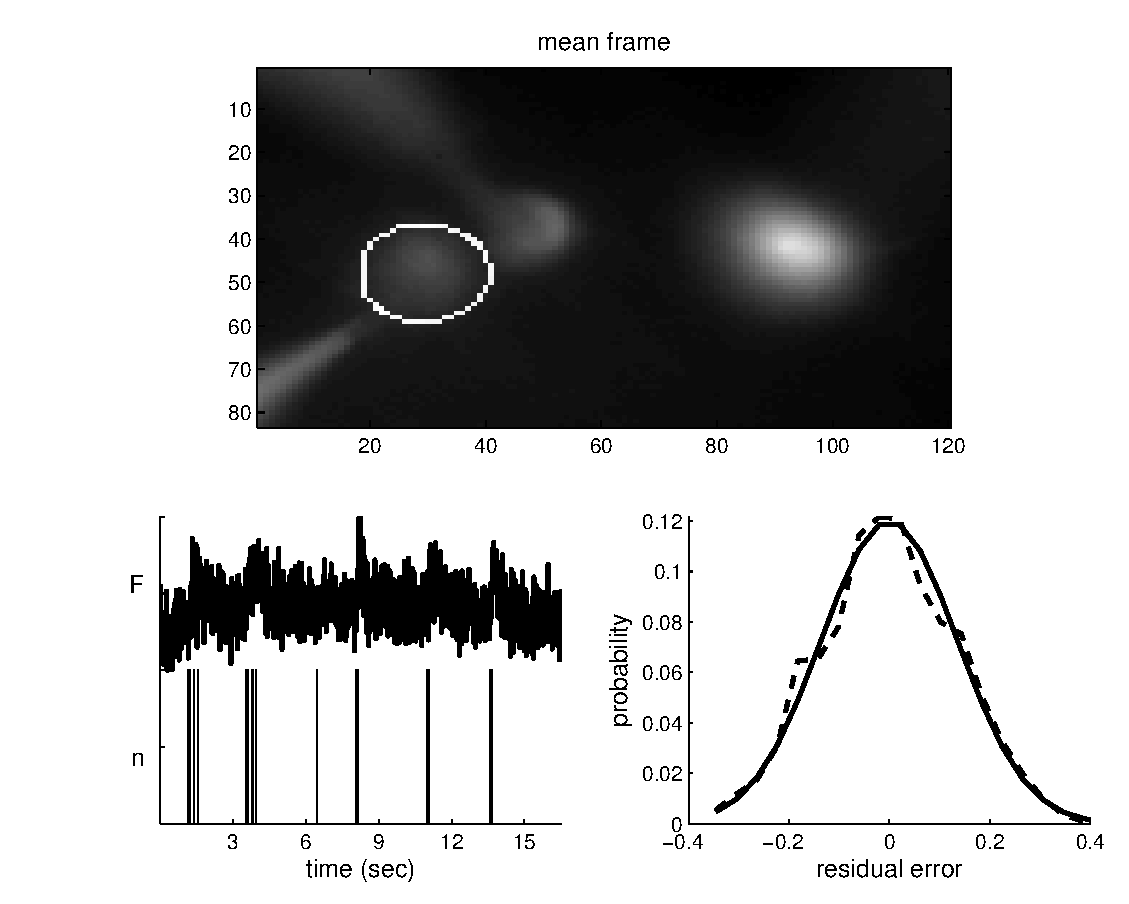
\includegraphics[width=.9\linewidth]{../figs/in_vitro_ex}
\caption{A typical in vitro data-set suggests that a reasonable first order model may be constructed by convolving the spike train with an exponential, and adding Gaussian noise. Top panel: the average (over frames) of a typical field-of-view.  Bottom left: spike train (black bars), convolved with an exponential (gray line), superimposed on the one-dimensional fluorescence time series (black line).  Bottom right: a histogram of the residual error between the gray and black lines from the bottom left panel (black line), and the best fit Gaussian (gray line).} \label{fig:in_vitro_ex}
\end{figure}

The above observations may be formalized as follows. Assume we have a 1-dimensional fluorescence trace, $\bF=(F_1, \ldots, F_T)$ from a neuron.  At time $t$, the fluorescence measurement, $F_t$ is a linear-Gaussian function of the intracellular calcium concentration at that time, $C_t$:

\begin{align} \label{eq:F}
F_t &= \alpha (C_t + \beta) + \sig \varepsilon_t, \qquad \varepsilon_t \overset{iid}{\sim} \mN(0,1)
\end{align}

\noindent The scale, $\alpha$, absorbs all experimental variables impacting the scale of the signal, including number of sensors within the cell, photons per change in intracellular calcium concentration per sensor, amplification of imaging system, etc.  Similarly, the offset, $\beta$, absorbs baseline calcium concentration of the cell, background fluorescence of the fluorophore, imaging system offset, etc.  The standard deviation, $\sig$, results from calcium fluctuations independent of spiking activity, fluorescence fluctuations independent of calcium, and imaging noise. The noise at each time, $\varepsilon_t$, is independently and identically distributed according to a standard normal distribution (i.e., Gaussian with zero mean and unit variance).  %These three parameters, and the Gaussianity of the noise,  correspond to a number of simplifying assumptions, that we will relax in Section \ref{sec:results}.  

We further assume that the intracellular calcium concentration, $C_t$, jumps after each spike, and subsequently decays back down to rest with time constant, $\tau$, yielding:

% $\tau (C_t-C_{t-1})/\Del = -C_{t-1} + n_t$.  Rearranging (and rescaling) a bit, we have:

\begin{align} \label{eq:C}
\tau \frac{C_t - C_{t-1}}{\Del} &= - C_{t-1} + n_t
\end{align}

\noindent where $\Del$ is the time step size --- which in our case, is the frame duration, or $1/$(frame rate) --- and $n_t$ indicates the number of times the neuron spiked at time $t$. %, and $\gam=1-\Del/\tau$. \footnote{This follows from writing \eqref{eq:C} as $\tau \frac{C_t - C_{t-1}}{\Del} = -C_{t-1} + n_t$.} 
Note that $C_t$ does not refer to absolute intracellular concentration of calcium but rather, a relative measure.  The assumed linearity of our model precludes the possibility of determining calcium in absolute terms (but see Section \ref{sec:nonlin} for a modified model).  The gray line in the bottom left panel of Figure \ref{fig:in_vitro_ex} corresponds to the putative $\bC$ of the observed neuron.  

To complete the ``generative model'' (i.e., a model from which we could generate simulations), we must also define the distribution from which spikes are sampled.  Perhaps the simplest first order description of spike trains is that at each time, spikes are sampled according to a Poisson distribution with some rate:

\begin{align} \label{eq:n}
	n_t \overset{iid}{\sim} \text{Poisson}(\lam \Del)
\end{align}

\noindent where $\lam \Del$ is the expected firing rate, and we have included $\Del$ to make $\lam$ be independent of the frame rate.  Thus, Eqs. \eqref{eq:F} -- \eqref{eq:n} complete our generative model.  


%Figure \ref{fig:schem} depicts a schematic illustration of this model. 

% \begin{figure}[h!]
% \centering 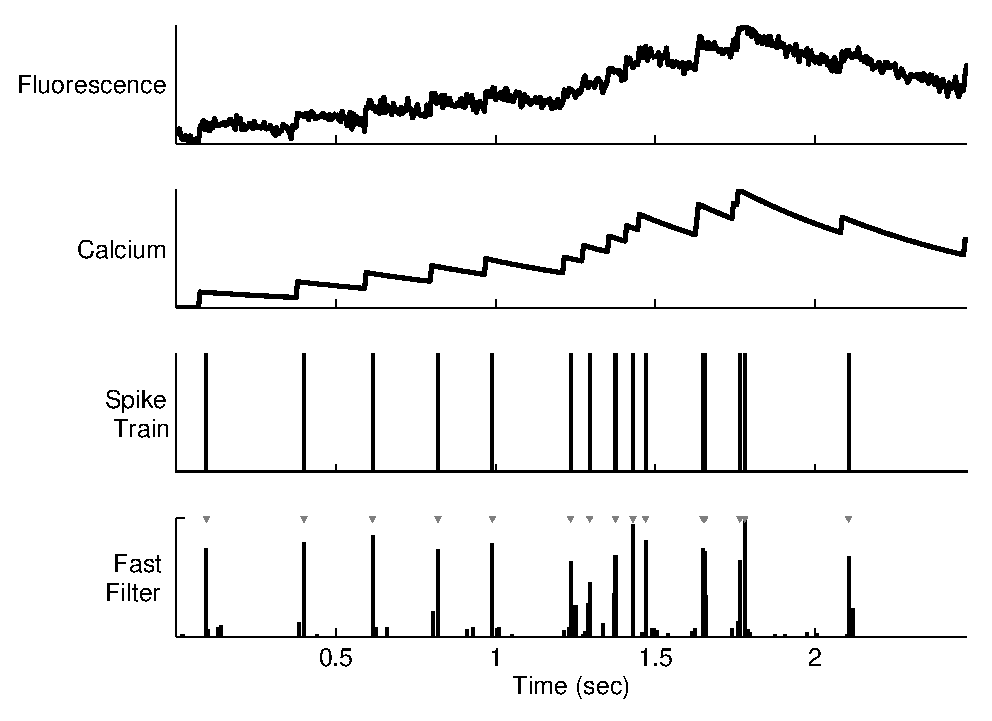
\includegraphics[width=.9\linewidth]{../figs/schem}
% \caption{A schematic illustrating our model. The spike train (bottom panel) is convolved with an exponential with time constant $\tau$ to obtain the calcium dynamics (middle panel).  The fluorescence observations are simply the calcium dynamics, plus zero mean Gaussian noise (with variance $\sig^2$). Parameters: $\Del=5$ msec, $\alpha=1$ photons/$\mu$M, $\beta=0$ unitless, $\sig=0.25$ photons, $\tau=100$ msec, $\lam=5$ Hz.} \label{fig:schem}
% \end{figure}


%relating spikes, $n_t$, baseline subtracted intracellular calcium concentration, denoted by $C_t$, and fluorescence measurements, $F_t$.  First, we assume a linear relationship between $F_t$ and $C_t$, with gaussian noise.  Second, we assume that $C_t$ jumps after each spike, and then decays according to some time constant.  Finally, we assume that spikes are distributed according to a Poisson process. The above assumptions lead to the follwoing model:

%. (1) spikes follow Poisson statistics with rate $\lam \Del$, (2) $C_t$ decays exponentially with decay $\gamma$ to baseline $\nu$, but jumps by $\rho$ after each spike, and (3) fluorescent observations are linear functions of $C_t$ with additive Gaussian noise with variance $\sig^2$.  Together, these assumptions imply the following model:

%\begin{align}
%\bF_t &= \balpha (C_t + \beta) +  \ve{\varepsilon}_t, \qquad &\ve{\varepsilon}_t \sim \mathcal{N}(\ve{0},\sig^2 \bI) \label{eq:obs} \\
%C_t  &= \gamma  C_{t-1} + n_t,  \qquad &n_t \sim \text{Poisson}(n_t; \lam \Del) \label{eq:trans}  
%\end{align}

%\noindent where $\balpha$ and $\beta$ set the fluorescence spatial filter and offset respectively, $\sig^2$ indicates the variance of the noise, and $\gamma$ sets the decay rate. 

%Note that   . To enforce identifiability, we will let $\balpha=1$ and $\beta=0$, without loss of generality, as explained below.




\subsection{Inference} \label{sec:inf}
\paragraph{FAst Non-negative Deconvolution (FAND) Filter}

Our goal here is to develop an algorithm to efficiently approximate $\hbn_{MAP}$.  The main contribution of this work demonstrating that we can substitute the Poisson distribution with an exponential distribution, reducing computational complexity from $O(k^T)$ to $O(T)$.  Formally, we replace Eq. \eqref{eq:C} with:

\begin{align} \label{eq:C2}
	C = \gam C_{t-1} + n_t, \qquad n_t \overset{iid}{\sim} \text{Exponential}(\lam \Del)
\end{align}

\noindent where the only difference between Eq. \eqref{eq:C} and Eq. \eqref{eq:C2} is the distribution on $n_t$.  Plugging this change into Eq. \eqref{eq:naht3} yields
%, by replacing the Poisson distribution on $\bn$ with an exponential distribution. Plugging this approximation into Eq. \eqref{eq:nhat4} yields:

\begin{align} \label{eq:obj2}
\bn^{FAND} &= \argmax_{n_t>0 \, \forall t}  \sum_{t=1}^T \bigg( \frac{1}{2 \sig^2}(F_t - \alpha(C_t + \beta))^2  + n_t \lam \Del \bigg) %, \qquad n_t \overset{iid}{\sim} \text{Exponential}(\lam \Del) %\an  \sum_{t=1}^T \left( \frac{1}{2 \sig^2}(\norm{\bF_t -\balpha (C_t + \beta)}^2  +  n_t  \lam \Del \right).
\end{align}

\noindent where the constraint on $\bn$ has been relaxed from  $n_t \in \mathbb{N}_0$ to $n_t \geq 0$ (since the support of an exponential distribution is the non-negative number line).  Note that this is a common approximation technique in the machine learning literature \cite{HastieFriedman01}, as it is the closest convex relaxation to its non-convex counterpart. While this convex relaxation makes the problem tractable, the ``sharp'' threshold imposed by the non-negativity constraint prohibits the use of standard gradient ascent techniques \cite{BoydVandenberghe04}. We therefore take an ``interior-point'' (or ``barrier'') approach, in which we drop the sharp threshold, and add a barrier term, which must approach $-\infty$ as $n_t$ approaches zero (e.g., $-\log n_t$) \cite{BoydVandenberghe04}.  By iteratively reducing the weight of the barrier term, we are guaranteed to converge to the correct solution \cite{BoydVandenberghe04}.  Thus, our goal is to efficiently solve:

\begin{align} \label{eq:eta}
\hbn_{\zzz} &= \argmin_{n_t \forall t}  \sum_{t=1}^T \left( \frac{1}{2 \sig^2}(F_t - \alpha(C_t + \beta))^2  +  n_t  \lam \Del - \zzz \log(n_t) \right),
\end{align}

Since spikes and calcium are related to one another via a simple linear transformation, namely, $n_t= C_t-\gam C_{t-1}$, we may rewrite Eq. \eqref{eq:eta} in terms of $\bC$:

\begin{align} 
\hbC_{\zzz} &= \argmin_{C_t - \gamma C_{t-1} \geq 0 \forall t} \sum_{t=1}^{T} \left( \frac{1}{2 \sig^2} (F_t -\alpha (C_t + \beta))^2  + (C_t - \gamma C_{t-1}) \lam \Del - \zzz \log(C_t - \gamma C_{-1}) \right). \label{eq:eta2}
\end{align}

\noindent The concavity of Eq. \eqref{eq:eta2} facilitates utilizing any number of techniques guaranteed to find the global optimum.  The fact that the argument of Eq. \eqref{eq:eta2} is twice differentiable, suggests that we use the Newton-Raphson technique. Importantly, the state-space nature of this problem yields a particularly efficient approach. Specifically, note that the Hessian is \emph{tridiagonal}, which is clear upon rewriting \eqref{eq:eta2} in matrix notation:

\begin{align} 
\hbC_{\zzz} %&= \argmin_{C_t - \gamma C_{t-1} \geq 0 \forall t} \sum_{t=1}^{T} \left( \frac{1}{2 \sig^2}\norm{\bF_t -\balpha (C_t + \beta)}^2  + (C_t - \gamma C_{t-1}) \lam \Del - \zzz \log(C_t - \gamma C_{-1} -\nu ) \right) \nonumber \\
&= \az  \frac{1}{2 \sig^2} \norm{\bF - \alpha (\bC +\beta)}^2 + (\bM \bC )\T \blam  - \zzz \log(\bM \bC)\T\ve{1},  \label{eq:eta3}
\end{align}

\noindent where $\ve{M} \in \mathbb{R}^{T \times T}$ is a bidiagonal matrix, $\bM \bC \geq \ve{0}$ indicates that every element of $\bM \bC$ is greater than or equal to zero, $\T$ indicates transpose, $\ve{1}$ is a $T$ dimensional column vector, $\blam=\lam \Del \ve{1}\T$, and $\log(\cdot)$ indicates an element-wise logarithm.  Note that Eq. \eqref{eq:eta3} follows from writing $\bn$ in terms of $\bM$ and $\bC$:
 
% such as Newton-Raphson, which, na\"{i}ely, requires inverting the Hessian (second derivative), an $O(T^3)$ operation.  
%We have therefore reduced the computational burden from exponential to polynomial in $T$.   However, by utilizing the structure of Eq. \eqref{eq:trans}, we can devise an algorithm that further reduces computation burden from polynomial in $T$ to \emph{linear} in $T$.  In particular, we note here that 
%, or, in matrix notation: 

\begin{align} \label{eq:M}
\ve{M} \bC = %- \bb=
\begin{bmatrix}
1 & 0  & 0 & \cdots & \cdots \\
1 & -\gamma & 0 & \cdots & \cdots \\
0 & 1 & -\gamma & 0 & \cdots  \\
\vdots & \vdots & \vdots & \vdots & \vdots  \\
0 & 0 & 0 & 1 & -\gamma
\end{bmatrix}
\begin{bmatrix}
C_1 \\ C_2 \\ \vdots \\ \vdots \\ C_T  
\end{bmatrix}
%-\begin{bmatrix}
%\nu/\rho \\ \nu/\rho \\ \vdots \\ \vdots \\ \nu/\rho 
%\end{bmatrix}
= 
\begin{bmatrix}
n_1 \\ n_2 \\ \vdots \\ \vdots \\ n_T
\end{bmatrix}
= \bn
\end{align}

%\noindent and $\ve{M} \in \mathbb{R}^{T \times T}$ is a bidiagonal matrix. Given Eq. \eqref{eq:M}, we may rewrite Eq. \eqref{eq:eta} only in terms of $\bC$ (i.e., not $\bn$):
%
%\begin{subequations}  
%\begin{align} 
%\hbC_{\zzz} &= \argmin_{C_t - \gamma C_{t-1} \geq 0 \forall t} \sum_{t=1}^{T} \left( \frac{1}{2 \sig^2}\norm{\bF_t -\balpha (C_t + \beta)}^2  + (C_t - \gamma C_{t-1}) \lam \Del - \zzz \log(C_t - \gamma C_{-1} -\nu ) \right) \nonumber \\
%&= \az  \frac{1}{2 \sig^2} \norm{\bF - \balpha (\trans{\bC} +\beta+\ve{1}\T)}^2 + \lam \Del (\bM \bC )\T \ve{1}  - \zzz \log(\bM \bC)\T\ve{1},  \label{eq:eta2}
%\end{align}
%\end{subequations}

Thus, a little bit of calculus yields our update algorithm for $\bC_z$:

%As \eqref{eq:eta2} is concave (it is identical to Eq. \eqref{eq:eta} with different notation), we may use any descent technique to find $\hbC_{\zzz}$.  We elect to use the Newton-Raphson approach: 

%, i.e., update $\widehat{\ve{C}}_{\zzz}$ by adding to it the solution to $\ve{H}\ve{C} = \ve{g}$, weighted by $0<s\leq1$, where $\ve{H}$ and $\ve{g}$ are the Hessian and gradient of the argument in \eqref{eq:goal2}.  The step size, $s$, ensures that the posterior converges, by enforcing an increase in the objective with each step. Therefore, we have: 

\begin{subequations} \label{eq:NR}
\begin{align}
\hbC_{\zzz} &\leftarrow \hbC_{\zzz} + s \bd \\
\bH \bd &= \bg \\
\ve{g} &= -\frac{\alpha}{\sig^2}(\bF -\alpha({\hbC\T}_{\zzz} + \beta)) + \ve{M}\T\blam - \zzz \ve{M}\T (\ve{M} \hbC_{\zzz})^{-1} \label{eq:g} \\
\ve{H} &= \frac{\alpha^2}{\sig^2} \ve{I} + \zzz \ve{M}\T (\ve{M} \hbC_{\zzz})^{-2} \ve{M} \label{eq:H}
\end{align}
\end{subequations}

\noindent where $s$ is the step size, $\bd$ is the step direction, and $\bg$ and $\bH$ are the gradient (first derivative) and Hessian (second derivative) of the argument in Eq. \eqref{eq:eta3} with respect to $\bC$, respectively, and the exponents indicate element-wise operations. Note that we use ``backtracking linesearches'', meaning that for each iteration, we find the maximal $s$ that is (i) between $0$ and $1$ and (ii) decreases the likelihood.

Typically, implementing Newton-Raphson requires inverting the Hessian, i.e., $\bd = \bH^{-1} \bg$, a computation consuming $O(T^3)$ time. Already, this would be a drastic improvement over the most efficient algorithm assuming Poisson spikes, which require $O(k^T)$ time (where $k$ is the maximum number of spikes per frame).  Here, because $\ve{M}$ is bidiagonal, the Hessian is tridiagonal, the solution may be found in $O(T)$ time via standard banded Gaussian elimination techniques (which can be implemented efficiently in Matlab using $\bH \backslash \bg$). In other words, the above approximation and inference algorithm reduces computations from exponential time to \emph{linear} time. We refer to this fast algorithm for solving \eqref{eq:obj2} the FAst Nonnegative Deconvolution (FAND) filter. 


\paragraph{Fast Wiener Filter}

Instead of replacing the Poisson distribution on spikes with an exponential, we can replace it with a Gaussian:

 \begin{align} \label{eq:C3}
	C = \gam C_{t-1} + n_t, \qquad n_t \overset{iid}{\sim} \mN(\lam \Del, \lam \Del)
\end{align}

\noindent which, when plugged into Eq. \eqref{eq:nhat3} yields

\begin{align} \label{eq:obj3}
\bn^{Wiener} &= \argmax_{n_t}  \sum_{t=1}^T \bigg( \frac{1}{2 \sig^2}(F_t - \alpha(C_t + \beta))^2  + 
 \frac{1}{2 \lam \Del}(n_t - \lam \Del)^2\bigg) 
\end{align}

Using the same tridiagonal trick as above, we can solve Eq. \eqref{eq:obj3} using Newton-Raphson once (since we have a quadratic problem here, see Appendix \ref{sec:wiener} for details).  Because we know only positive spikes are possible, at times we will also consider, $[$Wiener$]_+$, which is the Wiener filter half-wave rectified, i.e., all sub-zero values are set to zero.  

\section{Results}

\clearpage\newpage
\subsection{Main Result}
The main result of this paper is that we can approximate $\bn_{MAP}$ in \emph{linear} time, whereas an exact solution would require exponential time. Fig. \ref{fig:wiener} shows two examples of running the FAND filter on simulated data.  On the left, the data is simulated according to Eqs. \eqref{eq:F} and \eqref{eq:C}, with a low expected firing rate (5 Hz).  The FAND filter performs very well (middle left panel): when spikes occured (gray downward facing triangles), the FAND filter's output is relatively high, and in the absence of a spike, the FAND filter's output is relatively low. The height of the ``spikes'' in $\bn_{FAND}$ can be thought of as the probability of a spike having occurred.  The Wiener filter does not perform as well on this data.  Specifically, $\bn_{Wiener}$ exhibits a ``ringing'' effect, in which the inference oscillates around zero in the absence of true spikes.  This occurs because negative spikes improve the inference, if negative spikes are allowed.  By constraining our inference to be non-negative (for the FAND filter), we completely circumvent this problem.  

It is unsurprising that the FAND filter significantly outperforms the Wiener filter when spiking is sparse, given that the exponential is a much better approximation to the Poisson in this regime (c.f. Figure \ref{fig:dist_comp}).  However, even in the fast firing rate scenario, where the Gaussian approximation is far more accurate, the FAND filter performs relatively well, as depicted in the right panels of Figure \ref{fig:wiener}.  Note however that the computational time for computing the FAND filter scales linearly with $T$, i.e. is $O(T)$, whereas the \nai ve implementation of the Wiener filter requires $O(T \log T)$ (but see Appendix \ref{sec:app} for an implementation of the Wiener for that only requires $O(T)$).  

\begin{figure}[H]
\centering 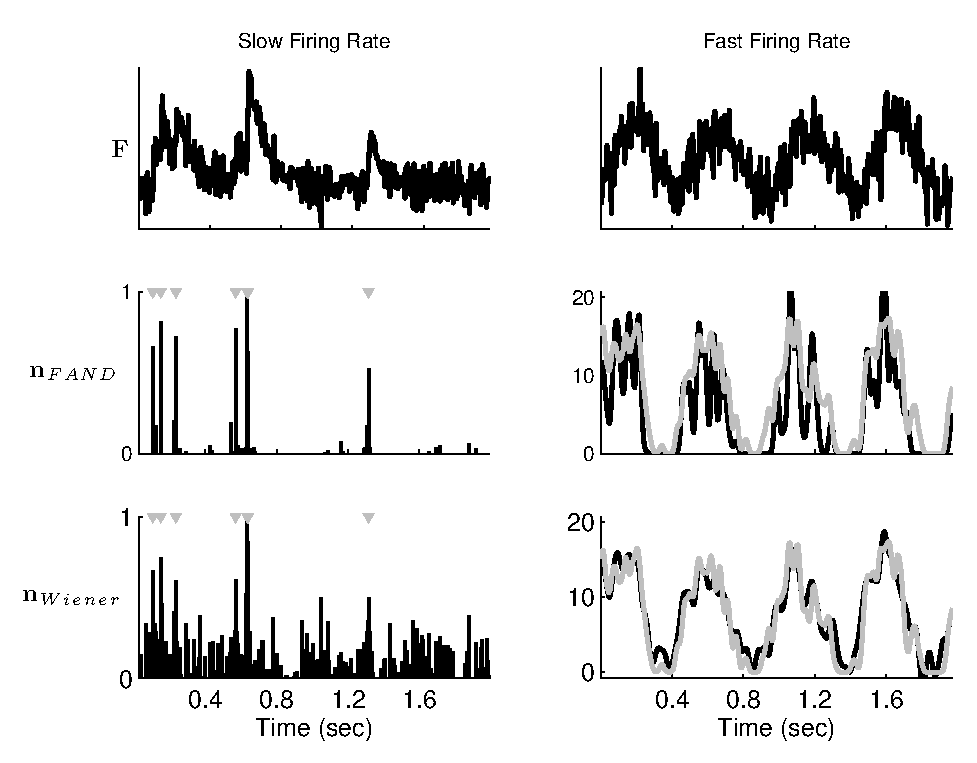
\includegraphics[width=.9\linewidth]{../figs/example_sim}
\caption{A simulation demonstrating that the FAND filter performs at least as well as the optimal linear (i.e., Wiener) filter. The left panels show that in the slow firing regime, the FAND filter outperforms the Wiener filter in terms of SNR.  This ``makes sense'', given that if a neuron is spiking according to a Poisson distribution with a slow rate, an exponential distribution is a better approximation than a Gaussian distribution, and the FAND filter approximates the spike train distribution with an exponential, versus the Wiener filter's Gaussian. The right panels show that both approximations are sufficient in the fast firing regime. Top left panel: fluorescence time series for a neuron with a slow firing rate.  Middle left panel: the FAND filter's inferred spike train.  Bottom left panel: Wiener filter's inferred spike train.  Note that (i) the Wiener filter does not impose a non-negativity constraint, and (ii) the effective SNR of the Wiener filter in this example is worse than the FAND filter's.  Top right panel: same as top left panel, for a neuron with a high firing rate.  Middle right panel: the FAND filter's inferred spike train smoothed with a Gaussian kernel for visualization purposes (black line), and the true spike train smoothed with the same Gaussian kernel (gray line).  Bottom right panel: same as middle right panel, but with the Wiener filter. Parameters for left panels: same as above.  Parameters for right panels: same as above, except: $\sig=8$ photons, $\lam=500$ Hz.} \label{fig:wiener}
\end{figure}

To quantify the relative quality of these inference algorithms in the sparsely spiking regime, we compute a number of distance measures between $\bn$ and our inferred $\hbn$: (a) cross correlation, (b) mean square error, and (c) signal-to-noise ratio (see Section \ref{sec:ass} for details). Figure \ref{fig:stats} (top panels) shows how the various algorithms (FAND in blue, Wiener in red, half-wave-rectified Wiener in green, dF/F in turquise) perform according to each of these measures, as a function of the noisiness of the data. Clearly, regardless of the variance of the noise, the FAND filter outperforms all other approaches considered here.   On the contrary, in the high firing rate regime, the Wiener filter is optimal, as expected (lower left panels).  Note that SNR is only an appropriate measure when there is at most one spike per image frame.  Finally, do demonstrate that our algorithms are indeed linear in the number of time steps, we show how computational time scales with $T$ (lower right panel) for each algorithm.


\begin{figure}[H]
\centering 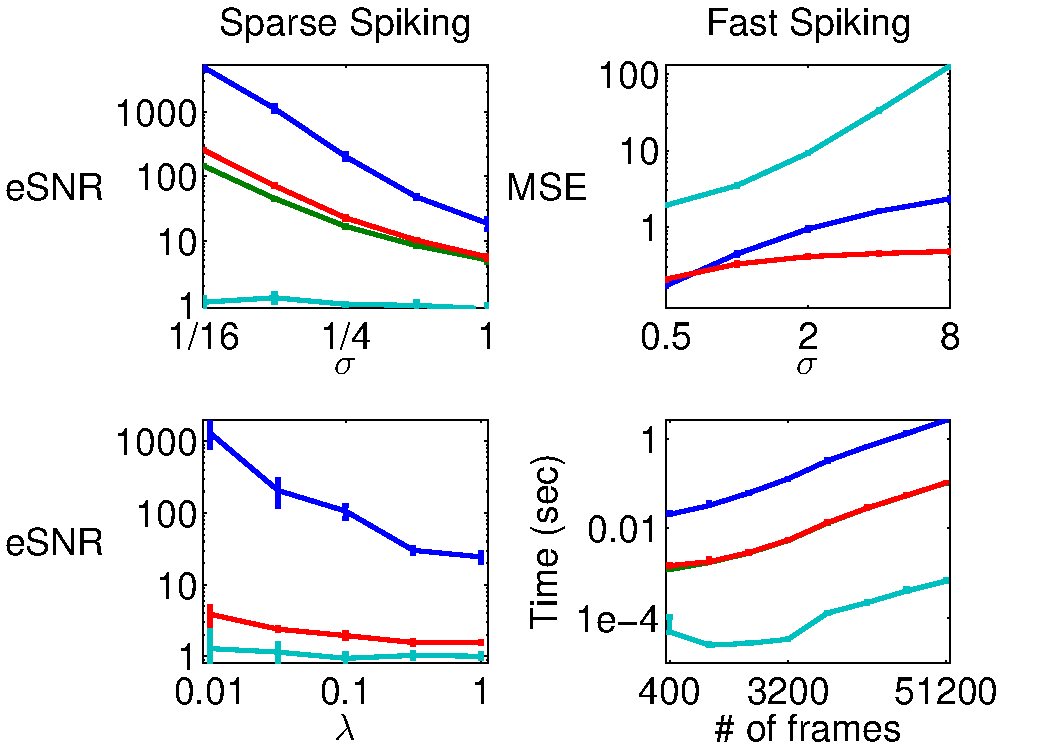
\includegraphics[width=.9\linewidth]{../figs/stats}
\caption{} \label{fig:stats}
\end{figure}


% To quantify the relative quality of these inference algorithms, Table \ref{tab:1} shows $R_{\hbn}$ and AUC for simulations like these, as well as computational time.  Clearly, the FAND filter is preferable to the Wiener filter, in that the FAND filter's performance is at least as good as the Wiener filter's, and requires less time.  
% 
% \begin{table}
% \caption{Simulated performance} \label{tab:slow}
% \centering
% \begin{tabular}{c|c|c|c|c|c}
% \multicolumn{6}{c}{Slow Firing Rate} \\ %\hline
% %Filter 			& $R_{\hbn}$ 	& $MSE$ 		& $SNR$ 		& $AUC$ & Time \\ \hline
% Filter & $R_{\hbn}$ & $MSE$ & $SNR$ & $AUC$ & Time \\ \hline 
FAND& 0.920 (0.009) & 0.006 (0.001) & 396.256 (91.462) & 6.315 (0.289) & 0.495 (0.020) \\ 
Wiener& 0.552 (0.012) & 0.024 (0.002) & 19.337 (1.508) & 6.485 (0.462) & 0.022 (0.001) \\ 
$[$Wiener$]_+$& 0.670 (0.010) & 0.017 (0.001) & 29.801 (2.436) & 6.485 (0.462) & 0.022 (0.001) \\ 
dF/F& -0.029 (0.009) & 0.067 (0.006) & 1.109 (0.222) & 0.853 (0.089) & 0.000 (0.000)
% %\end{tabular}
% %\end{table}
% \\ \hline \\
% %\begin{table}
% %\caption{Fast Firing Rate} \label{tab:fast}
% %\centering
% %\begin{tabular}{c|c|c|c|c|c}
% \multicolumn{6}{c}{Fast Firing Rate} \\ %\hline
% %Filter 			& $R_{\hbn}$ 	& $MSE$ 		& $SNR$ 		& $AUC$ & Time \\ \hline
% Filter & $R_{\hbn}$ & $MSE$ & $SNR$ & $AUC$ & Time \\ \hline 
FAND& 0.752 (0.005) & 67.689 (1.703) & NaN (NaN) & NaN (NaN) & 0.765 (0.016) \\ 
Wiener& 0.916 (0.001) & 15.323 (0.141) & NaN (NaN) & NaN (NaN) & 0.243 (0.005) \\ 
$[$Wiener$]_+$& 0.916 (0.001) & 15.323 (0.141) & NaN (NaN) & NaN (NaN) & 0.243 (0.005) \\ 
dF/F& 0.006 (0.005) & 385.433 (2.399) & NaN (NaN) & NaN (NaN) & 0.000 (0.000)
% \end{tabular}
% % }
% % \end{multicols}
% \end{table}

Finally, often one is interested in understanding the relationship between spike trains and the environment.  Therefore, we simulated a neuron whose spiking activity was a function of a 5-dimensional external stimulus.  More specifically, we let $\blam = \bk\T \bx$, where $\bk$ is a 5-dimensional linear kernel, and $\bx = (\bx_1, \ldots, \bx_T)$ is the stimulus, and $P(n_t)=$Poisson($\lam_t \Del$).  We then computed the maximum likelihood estimate of the linear kernel, $\hbk=\hbn \bx\T (\bx \bx\T)^{-1}$.  Importantly, the simulation was constructed to incorporate both sparse spiking and fast spiking periods, much like sensory neurons have periods of quiescence, followed by stimulus driven bursts.  Thus, neither the FAND filter nor the Wiener filter's assumptions are entirely appropriate. Figure \ref{fig:kernel} shows the results of this simulation.  The true kernel, kernel estimated using the true spike times, and kernel estimated using the FAND filter, are nearly overlapping (black, gray, and blue lines, respectively).  The kernel estimated using the Wiener filter output, however, is effectively flat (red line). Post-hoc half-wave rectification of the Wiener filter output does not improve its ability to estimate this kernel (green line --- completely obscured by the unrectified Wiener filter output).  Finally, dF/F does not yield anything useful at all (turquoise line).  

\begin{figure}[H]
\centering 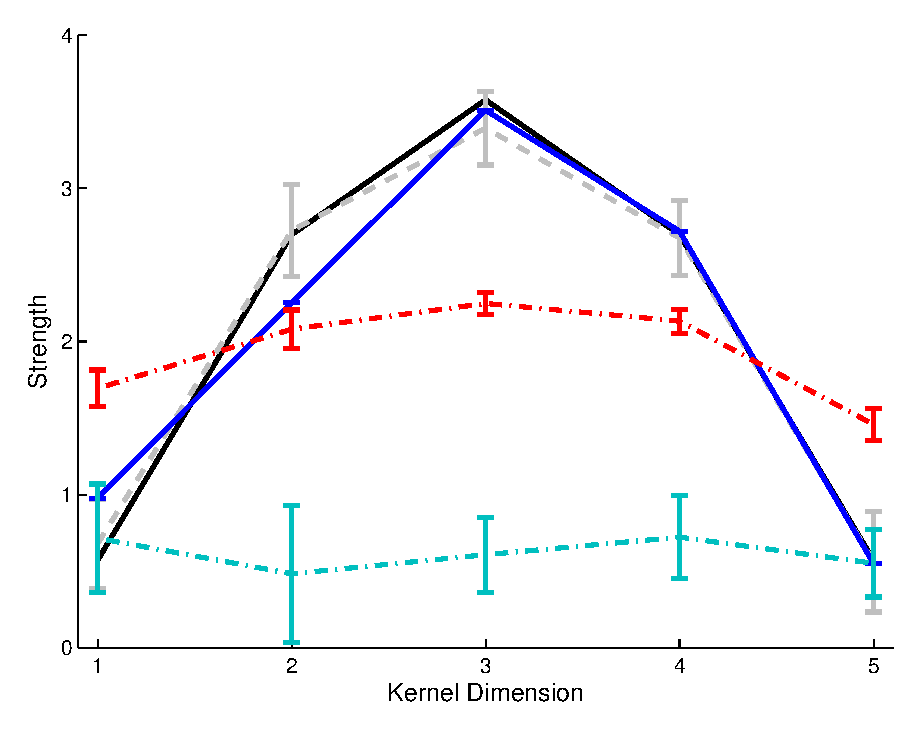
\includegraphics[width=.9\linewidth]{../figs/kernel}
\caption{XXX. Parameters: $T=800$, $\Del=5$ msec, $\alpha=1$, $\beta=0$, $\tau=100$ msec, $x_{i,t} \sim \mU(0,0.2)$,  $\sig=1/4$.} \label{fig:kernel}
\end{figure}


%The correlation coefficient between $\bn_{FAND}$ and $\bn$ versus $\bn_{Wiener}$ and $\bn$ for this example is $0.92$ versus $0.57$.  Thresholding $\bn_{Wiener}$ after inference improves the correlation coefficient to $0.69$.  Running this simulation many times demonstrates that these results are typical: $\bn_{FAND}$ always outperforms $\bn_{Wiener}$, whether or not it $\bn_{Wiener}$ thresholded.  



\clearpage\newpage
\subsection{Comparison with Wiener filter}
When the observed neuron is spiking quickly, the Poisson distribution may be well approximated by a Gaussian distribution, suggesting that the Wiener filter may be optimal in this regime.  But the exponential approximation of a Poisson is also very accurate in the fast spiking regime.  To compare these two strategies, we simulated a fast spiking neuron, where the expected number of spikes per bin exceeds 10 (Fig. \ref{fig:FastSpiking}). In this scenario, both the Wiener filter and our fast filter perform approximately equally well.  Both filters infer peaks in the firing rate that are obscured by the low-pass filter properties of the calcium dynamics. Thus, it seems from this analysis that regardless of the firing rate of the observable neuron, (1) filtering the signal may provide valuable information, and (2) our fast filter performs at least as well as the Wiener filter, without requiring more computational time.


\newpage \begin{figure}[H]
\centering 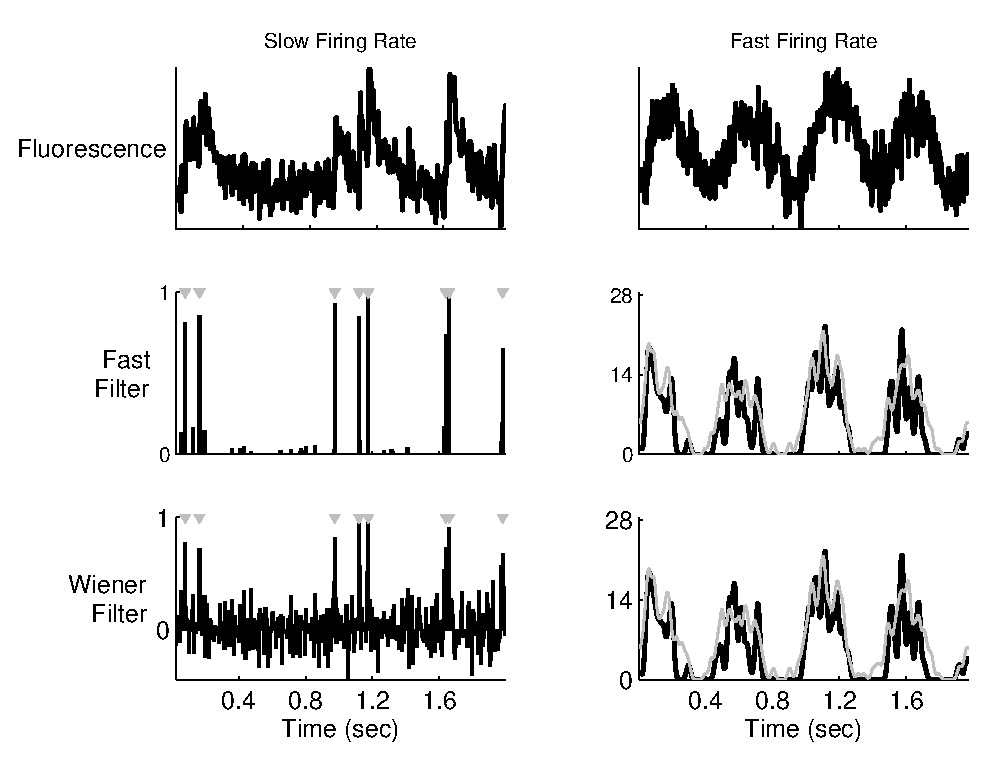
\includegraphics[width=.9\linewidth]{../figs/wiener}
\caption{A simulation demonstrating that the fast filter performs at least as well as the optimal linear filter. The left panels show that in the slow firing  regime, the fast filter --- which approximates the Poisson distribution governing spiking with an exponential distribution  --- outperforms the Wiener filter --- which approximates the Poisson distribution with a Gaussian.  The right panels show that both approximations are sufficient in the fast firing regime. Top left panel: fluorescence time series for a neuron with a slow firing rate.  Middle left panel: the fast filter's inferred spike train.  Bottom left panel: Wiener filter's inferred spike train.  Note that (i) the Wiener filter does not impose a non-negativity constraint, and (ii) the effective SNR of this filter in this example is higher than the fast filter's.  Top right panel: same as top left panel, for a neuron with a high firing rate.  Middle right panel: the fast filter's inferred spike train smoothed with a Gaussian kernel for visualization purposes (black line), and the true spike train smoothed with the same Gaussian kernel (gray line).  Bottom right panel: same as middle right panel, but with the Wiener filter. Parameters for left panels: same as above.  Parameters for right panels: same as above, except: $\sig=8$ a.u., $\lam=500$ Hz.} \label{fig:wiener}
\end{figure}

%\newpage \begin{figure}[H]
%\centering 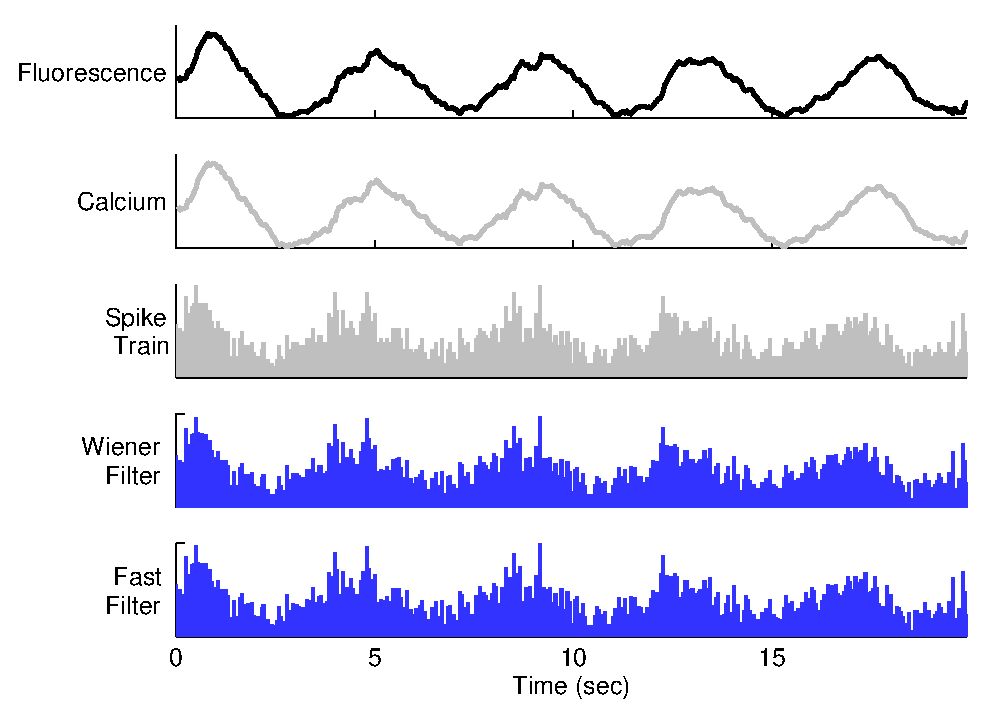
\includegraphics[width=.9\linewidth]{FastSpiking}
%\caption{Comparing the Wiener filter and our fast filter for a fast spiking neuron.  In this scenario, the two filters perform approximately equally well. Note that both recover fast fluctuations in the firing rate that are smoothed out by the calcium dynamics. Conventions as in Fig. \ref{fig:schem}.  Actual and inferred spike trains were normalized similarly, to ease comparisons. Parameters: $\gamma=0.94$, $\nu=0$, $\rho=1$, $\sig=0.3$, $\lam=100$ (modulated by a sinusoid), $\Del=0.05$ msec.} \label{fig:FastSpiking}
%\end{figure}




\clearpage\newpage
\subsection{Spatial Filtering}
In the above, we assumed a one-dimensional (1-D) observation, $\bF$.  The raw data, however, is actually a series of multidimensional images. To get the 1-D time-series, two pre-processing steps are required.  First, for each neuron, one must define a region-of-interest (ROI), essentially assigning sets of pixels to neurons. This yields a vector time-series for each neuron, $\vbF_t \in \Real^m$.   Second, one must project the $m-$D observations into a 1-D time-series.  Typically, this step is performed by averaging all the pixels within the ROI.  In theory, one can improve on this uniform averaging by estimating the optimal spatial filter. Here, we provide details on how to incorporate this second step (projecting the $m-$D observations into 1-D) into our fast filter. First, we replace Eq \eqref{eq:obj} with:

\begin{align}
\vbF_t &= \ve{\alpha} C_t + \ve{\beta} +  \ve{\Sig} \ve{\varepsilon}_t, \qquad \varepsilon_t \sim \mathcal{N}(\ve{0},\bI) \label{eq:Obs} 
\end{align}

\noindent where $\vbF_t$, $\ve{\alpha}$, and $\beta$ are all $m$ dimensional column vectors, $\ve{\Sig}$ is the covariance matrix, and $\ve{\varepsilon}_t$ is an $m-$dimensional standard normal random vector. $\Alpha$ now represents the optimal spatial filter, and $\Beta$ represents the baseline for each pixel.  Our goal then is to estimate $\Alpha$ and $\Beta$, to provide maximal information about the underlying spike train.  We would expect this optimal spatial filtering improve the effective SNR after filtering in many situations.  For example, if certain pixels are anti-correlated with others, a uniform spatial filter would average out those differences, whereas the optimal filter would take advantage of that information.    

To estimate $\Alpha$ and $\Beta$, we first plug 
%Then, plugging %To estimate the optimal spatial filter, first we assume that both $\bn$ and $\bC$ are known.  Then, letting $\ve{\eta}_v=[\gam \ve{\Alpha}, \nu \Alpha + \Beta, \rho \Alpha]'$, we see that the parameters are again unidentifiable.  This time, we let $\nu=0$ and $\rho=1$, yielding $\ve{\eta}_v=[\gam \ve{\Alpha}, \Beta,\Alpha]'$.  Then, plugging 
Eqs \eqref{eq:Obs} and \eqref{eq:trans} into \eqref{eq:par1}, to obtain:

\begin{align} 
\vec{\bth} &=\argmax_{\vec{\bth} \in \vec{\bTh}} - \frac{T}{2} \log (2\pi|\ve{\Sig}|) + T\log (\lam \Del) -  \lam \Del \bn' \ve{1} \nonumber\\
&-\frac{1}{2} \sum_{t=1}^T (\vbF_t - \ve{\alpha} (\gamma \hC_{t-1} -\nu  - \rho \hn_t) - \ve{\beta})' \ve{\Sig}^{-1} (\vbF_t - \ve{\alpha} (\gamma \hC_{t-1} -\nu  - \rho \hn_t) - \ve{\beta}) %\nonumber \\
\end{align} 

\noindent where $| \cdot |$ indicates the determinant. By pre-whitening the observation matrix, $\vbF=[\vbF_1, \vbF_2, \ldots, \vbF_T]$, we can estimate the covariance matrix by the identity, i.e., $\ve{\Sig}=\ve{I}$.   Without loss of generality, we may assume that $\nu=0$ and $\rho=1$, similar to our assumption of $\alpha=1$ and $\beta=0$ above. This leaves $\gamma$, $\Alpha$, and $\Beta$. Assuming that $\gamma$ is known (or estimated from the raw fluorescence signal, as we did above), we have: 

\begin{align}
\widehat{\ve{\eta}}_v = \argmax_{\norm{\ve{\eta}_v} <1} \norm{\vbF - \ve{\eta}_v \bX_v}^2 \label{eq:Par}
%\ve{\eta}_v &=\argmax_{\ve{\eta}_v, \, 0 < \gamma < 1} %- \frac{T}{2} \log (2\pi|\ve{\Sig}|) + T \log (\lam \Del) -\lam \Del \bn'\ve{1} 
%-(\vbF -\ve{\eta}_v \bX_v) ' \ve{\Sig}^{-1}   (\vbF - \bX \bth_v) \label{eq:Par}
\end{align}

\noindent where $\ve{\eta}_v=[\Alpha, \, \Beta]$, and $\bX_v=[\gamma \bC + \bn, \, \ve{1}]'$. Note that we have constrained the norm of $\ve{\eta}_v$, which is necessary because otherwise there is a free scale between $\bX_v$ and $\ve{\eta}_v$.  Problems of the form as in Eq \eqref{eq:Par} are known as ``trust region subproblems''.  Fortunately, many algorithms for solving such a problem are available \cite{Fortin00}. 


\begin{figure}[H]
\centering 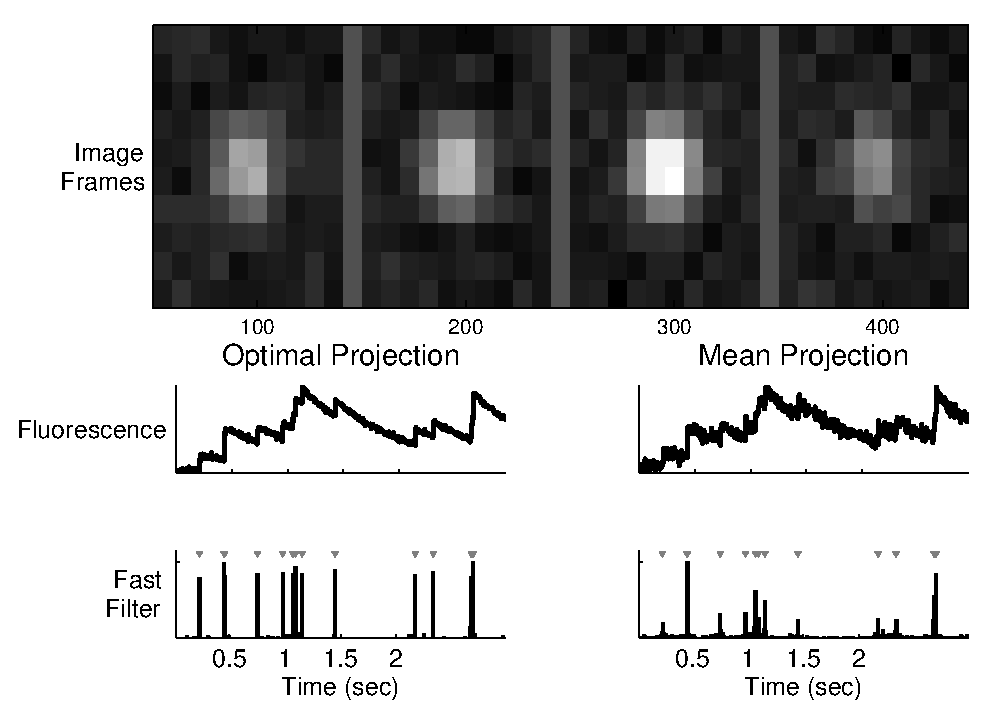
\includegraphics[width=.9\linewidth]{../figs/spatial}
\caption{A simulation demonstrating that using a better spatial filter can significantly enhance the effective SNR (see Supplementary Movie 1 for the full movie associated with this simulation).  Top: five movie frames, equally spaced from the entire move.  Middle left: projection of the entire movie onto the optimal spatial filter, yielding a 1D fluorescence time series, with a small SNR. Bottom left: fast filter's inferred spike train using the optimal spatial filter.  Middle right: projection of the entire movie onto the ``mean'' spatial filter, yielding a 1D fluorescence time series with a large SNR. Bottom right: fast filter's inferred spike train using the mean spatial filter. Parameters different from Fig \ref{fig:schem}: $\balpha$ is a mixture of two Gaussian kernels, each with the same mean, but different variances and component coefficients (see main text for details). $\bbeta=1$.} \label{fig:spatial} \end{figure} 

\begin{figure}[H]
\centering 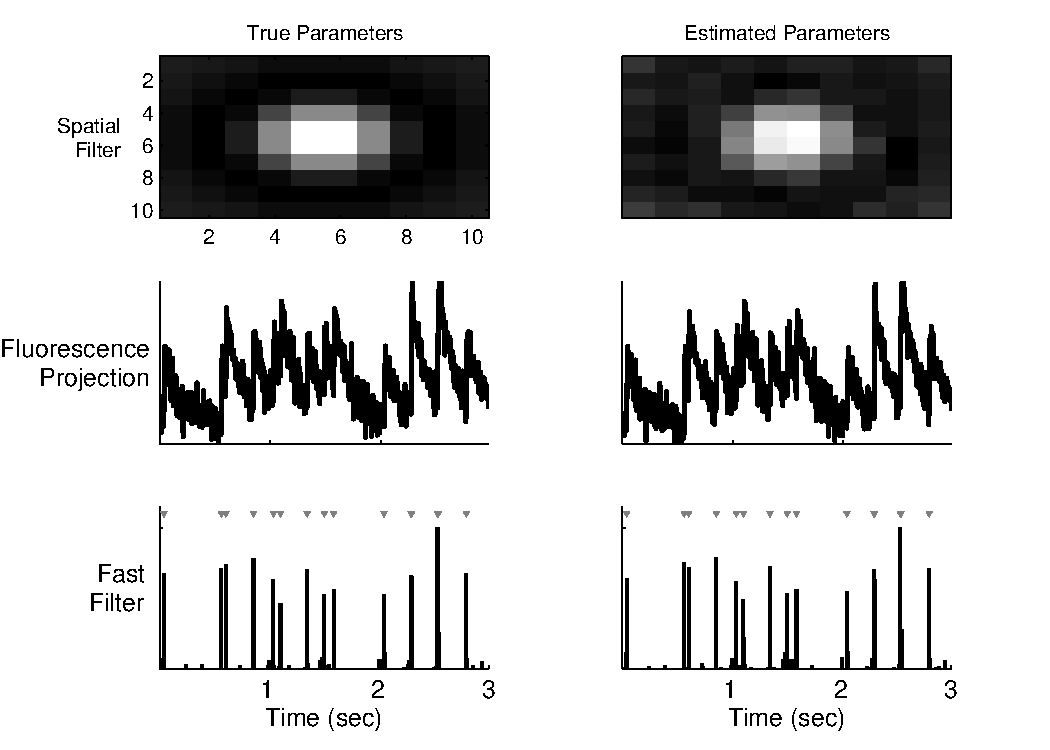
\includegraphics[width=.9\linewidth]{../figs/spatial_EM}
\caption{A simulation demonstrating that given only the fluorescence movie, the parameters may be estimated, and the spike train inferred (c.f. Supplementary Movie 2). Top left panel: true spatial filter.  Middle left panel: projection of movie onto true spatial filter. Bottom left panel: inferred spike train using true parameters. Right panels: same as left except estimating parameters.  $\balpha$ initialized with SVD.  $\bbeta$ initialized with $\ve{0}$.  $\lam$ and $\sig$ were initialized at double their true value.  $\tau$ was assumed known. Parameters same as above.} \label{fig:spatial_EM}
\end{figure}


%\subsection{Learning} \label{sec:est}
%In the above, we assumed that the parameters governing our model, $\vth=\{\alpha, \beta, \sig, \gam, \nu, \rho. \lam\} \in \ve{\Theta}$,  %=\Real^5_+$ (because all these parameters are necessarily non-negative)
were known. In general, however, these parameters may be estimated from the data. To find the maximum likelihood estimator for the parameters, $\hvth$, we must integrate over the unknown variable, $\zT$. However, integrating over all possible spike trains is typically approximated by Monte Carlo approaches, which is relatively slow. Thus, one often approximates: % the integral with the most likelihood estimate of $\zT$ \cite{??}, yielding:

%\begin{subequations} \label{eq:par}
\begin{align} \label{eq:par1}
\widehat{\bth} &= \argmax_{\bth \in \ve{\Theta}} \iint P(\bF|\bC, \bn, \bth) P(\bC, \bn | \bth) d\bn d\bC  \approx \argmax_{\bth \in \ve{\Theta}}P(\bF| \hCm, \hnm, \bth) P(\hCm, \hnm | \bth)
\end{align}

\noindent where $\hnm=[\hn_1, \ldots, \hn_T]$ is estimate of $\hnm$ from the inference algorithm described above ($\hCm$ is defined similarly). The approximation in \eqref{eq:par} is good whenever the likelihood is very peaky, meaning that most of the mass is around the MAP sequence.\footnote{The approximation in \eqref{eq:par} may be considered a first-order Laplace approximation}  In particular, for state-space models, one often approximates the integral in \eqref{eq:par} with the Viterbi path, i.e., the MAP path of the hidden states \cite{Rabiner89}. Finding the Viterbi path is often far easier than solving the integral in \eqref{eq:par}, as in the case here.  Due to the state space nature of the above model (Eqs \eqref{eq:obs} and \eqref{eq:trans}), the optimization in Eq \eqref{eq:par1} simplifies significantly.  More specifically, we can write the argument from the left-hand-side of Eq \eqref{eq:par1} as a product of terms that we have defined in our model:

 \begin{align} \label{eq:par2}
P(\bF| \hCm, \hnm, \bth) P(\hCm, \hnm | \bth) &= \prod_{t=1}^T P(F_t | \hC_t, \alpha, \beta,\sig) P(\hC_t | \hC_{t-1}, \hn_t, \gamma) P(\hn_t | \lam)
\end{align}

\noindent Thus, this likelihood is jointly concave in all the parameters.  To solve for $\{\alpha,\beta,\sig\}$, we solve:

\begin{align} 
\{\halpha, \hbeta, \hsig\} &= \argmax_{\alpha, \beta, \sig > 0} \sum_{t=1}^T \log P(F_t | \hC_t, \alpha, \beta, \sig) \nonumber \\
&=  \argmax_{\alpha, \beta, \sig > 0} -\frac{T}{2} \log (2 \pi \sig^2)  - \frac{1}{2\sig^2} \sum_{t=1}^T (F_t - \alpha \hC_{t} - \beta )^2 \nonumber \\
&=   \argmax_{\alpha, \beta, \sig > 0} -\frac{T}{2} \log (2 \pi \sig^2)  - \frac{1}{2\sig^2} \norm{\bF- \hbX \ve{\eta}}^2 \label{eq:lik2}
%P(\bF | \hCm, \alpha, \beta, \sig) &= \prod_{t=1}^T P(F_t | \hC_t, \alpha, \beta, \sig) = \prod_{t=1}^T \frac{1}{\sqrt{2 \pi \sig^2}} \exp \left\{-\frac{1}{2\sig^2} (F_t - \alpha \hC_t - \beta )^2\right\}, \label{eq:lik}% \nonumber \\
%&= \prod_{t=1}^T \frac{1}{\sqrt{2 \pi \sig^2}} \exp \left\{-\frac{1}{2\sig^2} \big[F_t - \alpha (\gamma \hC_{t-1} + n_t) - \beta \big]^2\right\} \label{eq:lik}
\end{align}

%\noindent which follows from Eq \eqref{eq:trans}. Taking the log of both sides yields:
%
% because $\hC_t$ is deterministic given $\hn_t$. Considering for a moment, only the quadratic term in Eq \eqref{eq:lik}, the terms can be reorganized:
%
%\begin{align}
%F_t - \alpha (\gamma \hC_{t-1} + \nu + \rho \hn_t) - \beta &= F_t - (\alpha \gamma) \hC_{t-1} - (\alpha \nu + \beta) - (\alpha \rho) \hn_t 
%\end{align}
%
%\noindent which emphasizes the over-parameterization in our model.  Thus, without loss of generality, we can assume that $\alpha=1$ and $\beta=0$. Taking logs in Eq \eqref{eq:lik} then yields:
%
%\begin{align} 
%\log P(\bF | \hnm, \bth) &=  -\frac{T}{2} \log (2 \pi \sig^2)  - \frac{1}{2\sig^2} \sum_{t=1}^T (F_t - \alpha \hC_{t} - \beta )^2 \nonumber \\
%&=  -\frac{T}{2} \log (2 \pi \sig^2)  - \frac{1}{2\sig^2} \norm{\bF- \hbX \ve{\eta}}^2
% \label{eq:lik2}
%\end{align}

\noindent where  $\ve{\eta}=[\alpha, \, \beta]$  and $\hbX_t=[\hC_{t}, \, 1]$.  Thus, solving for $\{\halpha,\hbeta\}$, is a constrained quadratic optimization problem, which can be solved efficiently using standard tools, such as Matlab's \texttt{quadprog}.  The variance may then be solved for analytically:

\begin{align} 
\widehat{\sig}^2 &= \frac{1}{T} \norm{\bF - \hbX \widehat{\ve{\eta}}}_2^2 \label{eq:sig}
\end{align}

\noindent Similarly, taking the log of the prior term, $P(\hnm | \bth )$ yields:

\begin{align} \label{eq:prior}
\log P(\hnm | \bth) =  \sum _{t=1}^T \log(\lam \Del)  -\lam \Del \hn_t =T (\lam \Del) - \lam \Del \hnm' \ve{1} 
\end{align}

\noindent Plugging Eqs \eqref{eq:lik2} and \eqref{eq:prior} back into Eq \eqref{eq:par1}, and noting that log is a monotonic function, we have:


%Given Eqs. \eqref{eq:obs} and \eqref{eq:trans}, we can write the above likelihood function as:

\begin{align} 
%\hvth &=\argmax_{\vth \in \ve{\Theta}}  \sum_{t=1}^T \left(- \frac{1}{2} \log (2\pi\sig^2)-\frac{1}{2\sig^2} (F_t - \gamma \hC_{t-1} -\nu  - \rho \hn_t)^2 \right) + \sum_{t=1}^T \big(\log (\lam \Del) -  \lam \Del n_t\big) \nonumber \\
\hvth &=\argmax_{\vth \in \ve{\Theta}} - \frac{T}{2} \log (2\pi\sig^2) - \frac{1}{2\sig^2} \norm{\bF - \hbX \ve{\eta}}_2^2 + T \log (\lam \Del) - \lam \Del \hnm' \ve{1} \label{eq:par} 
%&=\argmin_{\vth}  \frac{T}{2} \log (2\pi\sig^2)  +  \frac{1}{2\sig^2} \norm{\bY + \ve{\eta} \bX}_2^2 + T \log (\lam \Del) - \lam \Del \bn' \ve{1} \label{eq:par} 
\end{align}
%\end{subequations}

\noindent %where %$\bY=\bF- \hnm$, 
%$\bX=[\hCm, \,  \ve{1},\,  \hnm]'$, $\ve{\eta}=[\gamma, \nu, \rho]'$, and $\hCm=[\hC_1, \hC_2, \ldots, \hC_{T-1}]'$ is the inferred calcium concentration using the algorithm described in Section \ref{sec:inf} (and $\hnm$ is defined in a similar fashion). Note that had we not fixed $\alpha=1$ and $\beta=0$, then we would have had $\ve{\eta}=[\alpha \gamma, \alpha \nu + \beta, \alpha \nu]$, and then these parameters would not have been identifiable.  
Estimating the parameters then separates into three log-concave problems.  In particular, solving for $\widehat{\ve{\eta}}$ is simply:

\begin{align} 
\widehat{\ve{\eta}} &= \argmin_{\ve{\eta},\: 0< \eta_1<1} \frac{1}{2} \norm{\bF - \hbX \ve{\eta}}_2^2 
=  \argmin_{\ve{\eta},\: 0< \eta_1<1} \frac{1}{2} \ve{\eta}' \bQ  \ve{\eta} - \bL'  \ve{\eta} \label{eq:m} 
\end{align}

\noindent where $\bQ=\hbX' \hbX$, and $\bL=\hbX' \bF$, and the constraint, $0<\eta_1<1$, ensures that the time constant is both non-negative and finite.  Eq \eqref{eq:m} may be solved using standard quadratic optimization tools, such as Matlab's \texttt{quadprog}.  

Unfortunately, the recursive nature of our algorithm makes solving for $\hbeeta$ in this manner unidentifiable. In particular, because both $\hbX$ and $\beeta$ can scale and shift $\bC$, alternating between inferring $\hbX$ and $\hbeeta$ does not converge (data not shown). However, this is not particularly problematic, because the fluorescence measurements are in arbitrary units. This unit arbitrariness suggests that $\bF$ may be scaled and shift without loss of generality. The prior term and non-negativity constraint on $\bn$, however, imposes small costs associated with scaling and shifting $\bn$ and $\bC$.  We therefore estimate $\beeta$ from the raw fluorescence trace.  More specifically, to estimate $\gamma$, we manually find a fluorescence sequence that seem to be decaying, estimate the time constant $\tau$, and let $\gamma=1-\Del/\tau$.  For $\nu$, we manually find a fluorescence sequence that seems to be near baseline, label it $[F_s,\ldots, F_t]$, and let $\nu=\frac{1}{t-s}\sum_{u=s}^t F_u$.  Finally, we estimate $\rho$ by letting it be equal to what we manually determine it be, by eye.  In practice, we have found that by first scaling and shifting $\bF$ to be between $0$ and $1$, subsequent traces from the same or different cells have very similar values for $\beeta$, and therefore, these parameters need not be tweaked much.  Furthermore, the effective signal-to-noise ratio (SNR) of the inferred spike train does not depend strongly on these parameters, in agreement with previous results \cite{YaksiFriedrich06}.  The other parameters, $\sig$ and $\lam$, can be solved for analytically:

\begin{align} 
\widehat{\sig}^2 &= \frac{1}{T} \norm{\bF - \hbX \widehat{\ve{\eta}}}_2^2 \label{eq:sig2}\\
\widehat{\lam} &=  \frac{1}{T \Del} \hnm' \ve{1} \label{eq:lam}
\end{align}

%\noindent where Eq. \eqref{eq:m} may be solved using standard linearly constrained quadratic programming (the constraint ensures that the time constant is both non-negative and finite), and the other two may be solved analytically. Importantly, when $\bn$ is unknown, $\widehat{\ve{\eta}}$ is not identifiable, as $\bY$ and $\ve{\eta}$ can both modify the offset and scale of $\bn$. Thus, we estimate $\ve{\eta}$ \emph{before} doing the analysis, and then hold it fixed throughout.  

%. Because the noise is Gaussian, $a$ and $\beta$ may be estimated using standard constrained quadratic programming:
% 
%\begin{subequations}
%\begin{align} \label{eq:m}
%\{\ha,\hbeta\}% &= \argmax_{a,\beta>0}\frac{1}{\sqrt{2 \pi} \sig} \exp \left\{ -\frac{1}{2} \left(\frac{F_t - a \widehat{C}_{t-1} - \widehat{n}_t - \beta}{\sig}\right)^2\right\} 
%= \argmin_{a,\beta>0} \sum_{t=1}^T (F_t - a \widehat{C}_{t-1} - \widehat{n}_t -\beta )^2 \\
%\widehat{\ve{\eta}} &= \argmin_{\bm>0} \norm{\bY + \bm \bX}_2^2. % = \argmin_{\bm>0}  \bm' \bX' \bX \bm  - 2 \bY' \bX \bm 
%\end{align}
%\end{subequations}
%
% Similarly, because $\varepsilon_t$ is Gaussian, we compute $\widehat{\sig}$ analytically using: 
%
%\begin{align}
%\widehat{\sig}^2 = \frac{1}{T} \norm{\bY + \widehat{\ve{\eta}} \bX}_2^2.
%\end{align}
%
%\noindent The parameter for the prior term is given by:
%
%\begin{align}
%\widehat{\lam} = \argmax_{\lam} P(\widehat{\ve{n}} | \lam) =  \argmax_{\lam} \log P(\widehat{\ve{n}} | \lam) =  \frac{T}{ \Del \bn' \ve{1}}
%\end{align}
%
%\noindent which follows from assuming that $p(\zT | \lT)$ is exponential in \eqref{eq:approx}.





\clearpage\newpage
\subsection{in vivo data}

\begin{figure}[H]
\centering 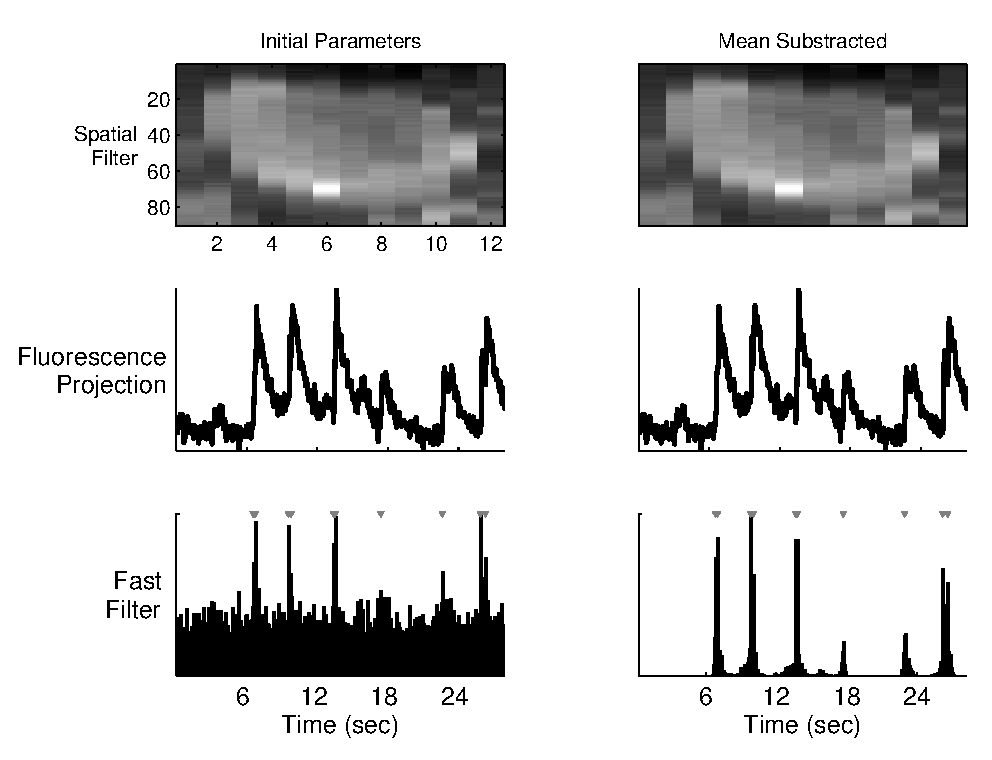
\includegraphics[width=.9\linewidth]{../figs/spatial_data}
\caption{Given only a fluorescence movie, recorded in vivo, we can learn the parameters necessary to correctly infer the spike trains. Left: mean frame.  Left: projection of movie onto mean frame. Left: the FANSI filter's inference.} \label{fig:spatial_data}
\end{figure}

%\begin{figure}[H]
%\centering 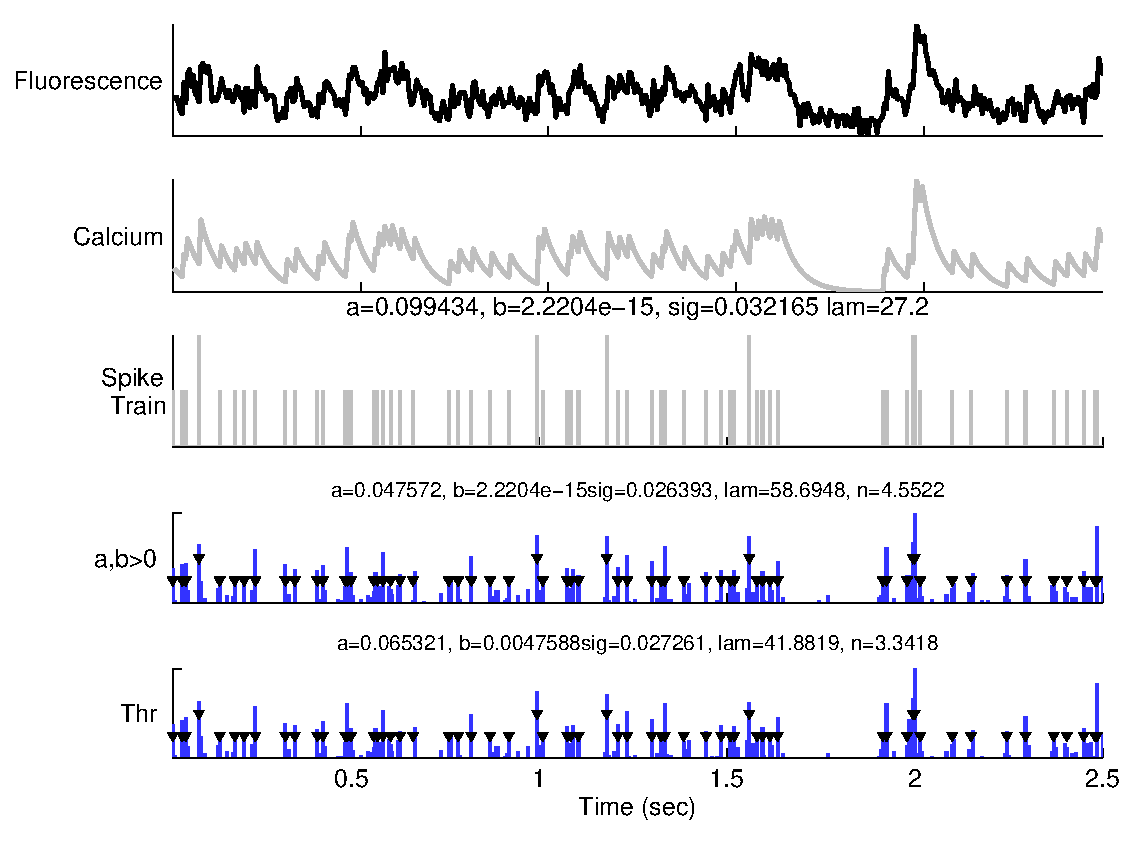
\includegraphics[width=.9\linewidth]{schem}
%\caption{distribution of errors in spike inference from real data} \label{fig:err}
%\end{figure}




\clearpage\newpage
\subsection{Overlapping spatial filters}
\begin{figure}[H]
\centering 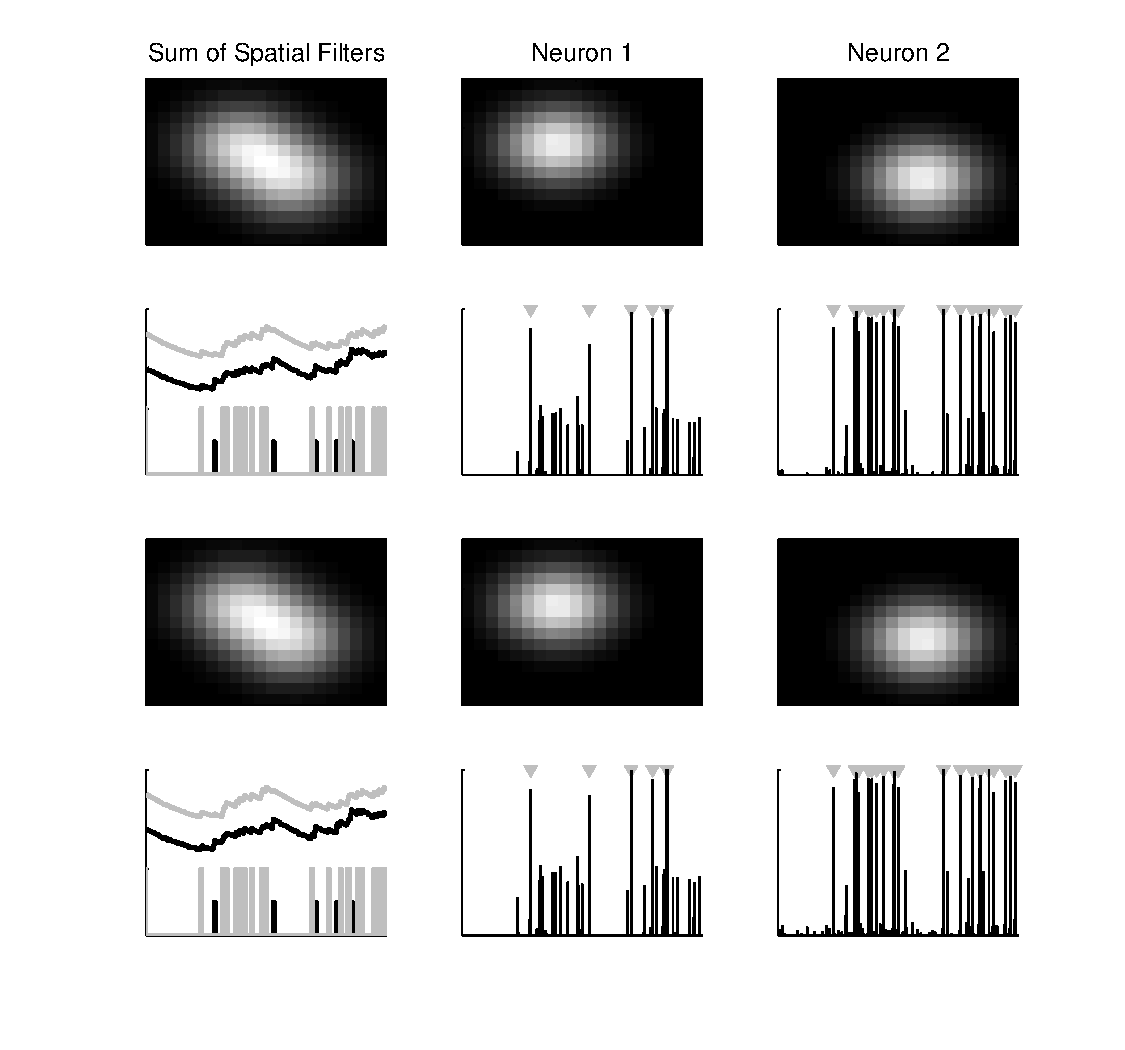
\includegraphics[width=.9\linewidth]{../figs/spatial_multi2}
\caption{Simulation showing that even when two neuron's spatial filters are largely overlapping, our inferencsame as spatial EM, but with 2 cells in ROI} \label{fig:spatial_multi}
\end{figure}

\begin{figure}[H]
\centering 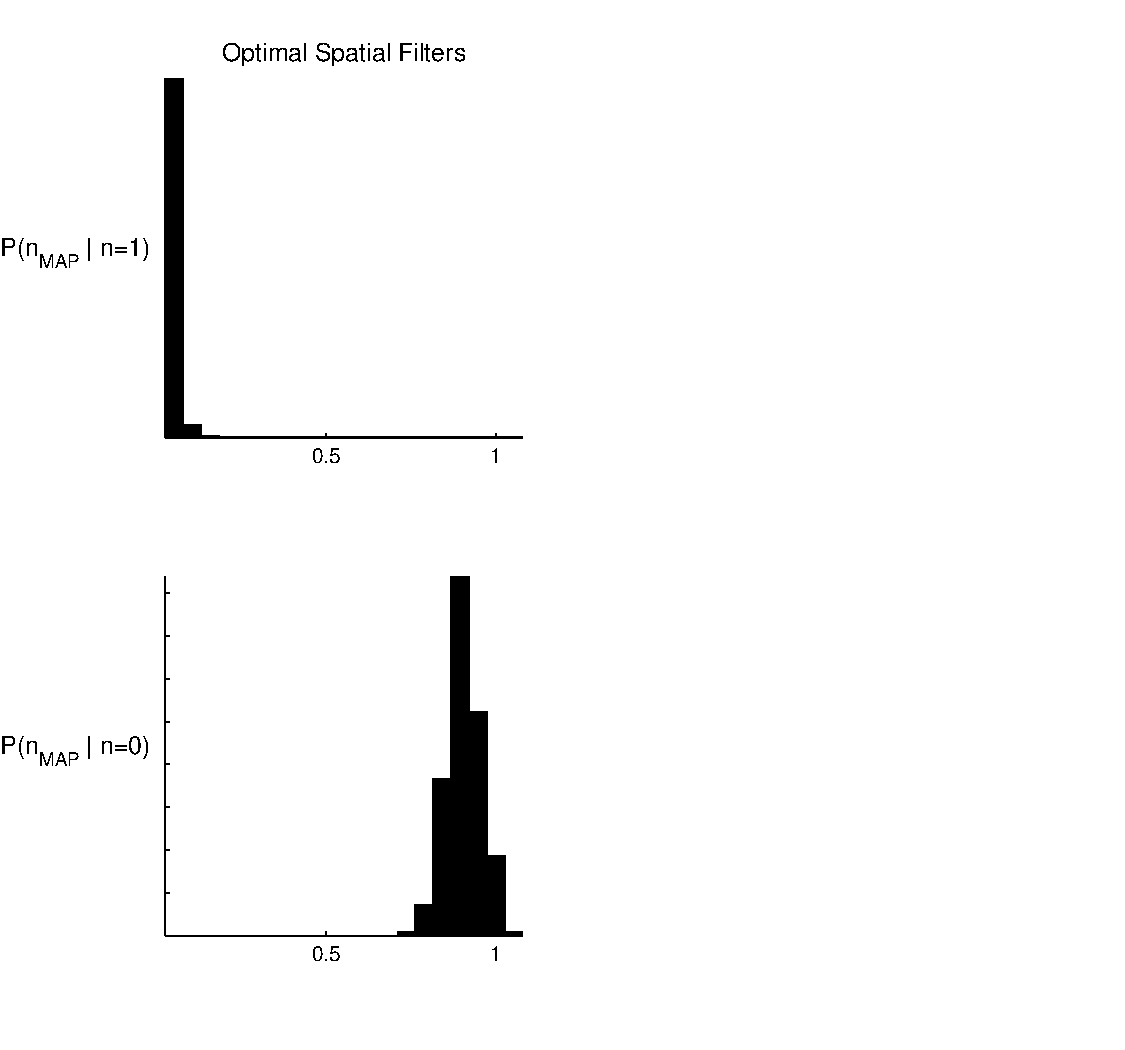
\includegraphics[width=.9\linewidth]{../figs/multi_hist1}
\caption{same as spatial EM, but with 2 cells in ROI} \label{fig:spatial_multi}
\end{figure}



\clearpage\newpage
\subsection{Analyzing a whole movie}

\newpage \begin{figure}[H]
%\centering 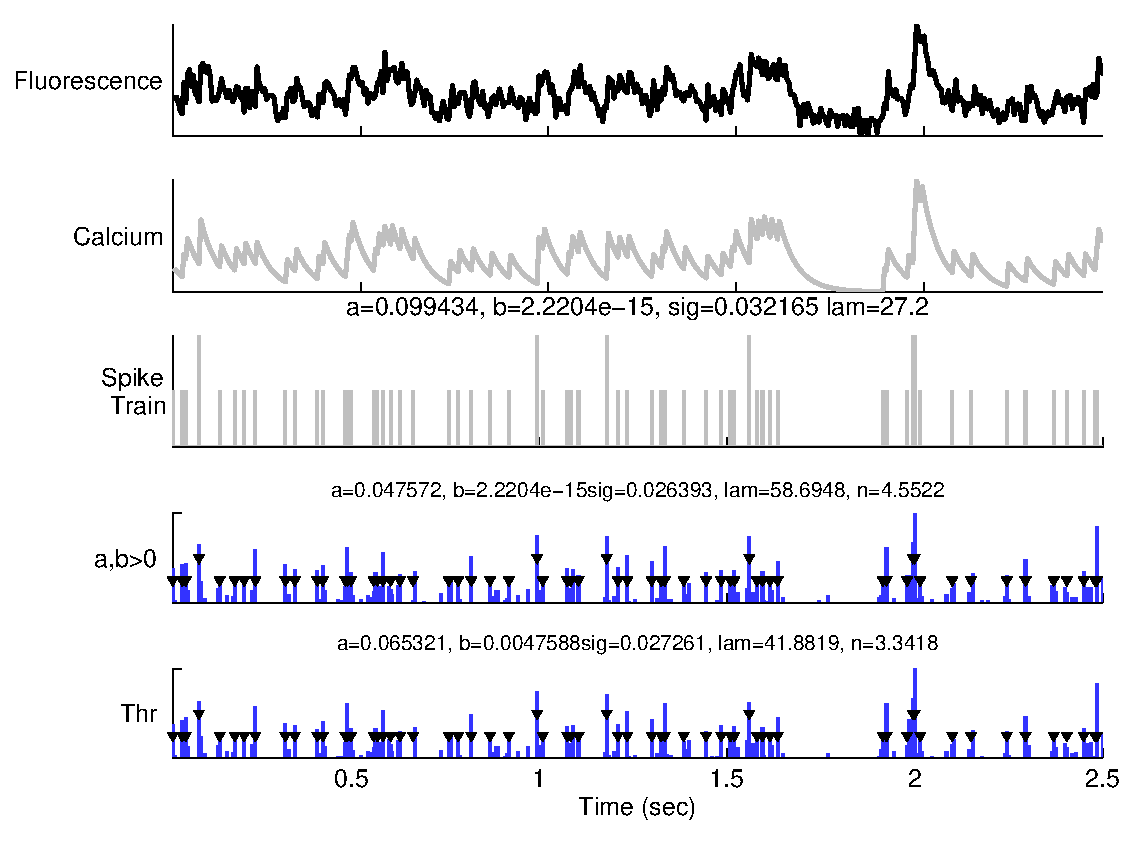
\includegraphics[width=.9\linewidth]{schem}
\caption{full movie, fully automated} \label{fig:spatial_full}
\end{figure}

\newpage \begin{figure}[H]
%\centering 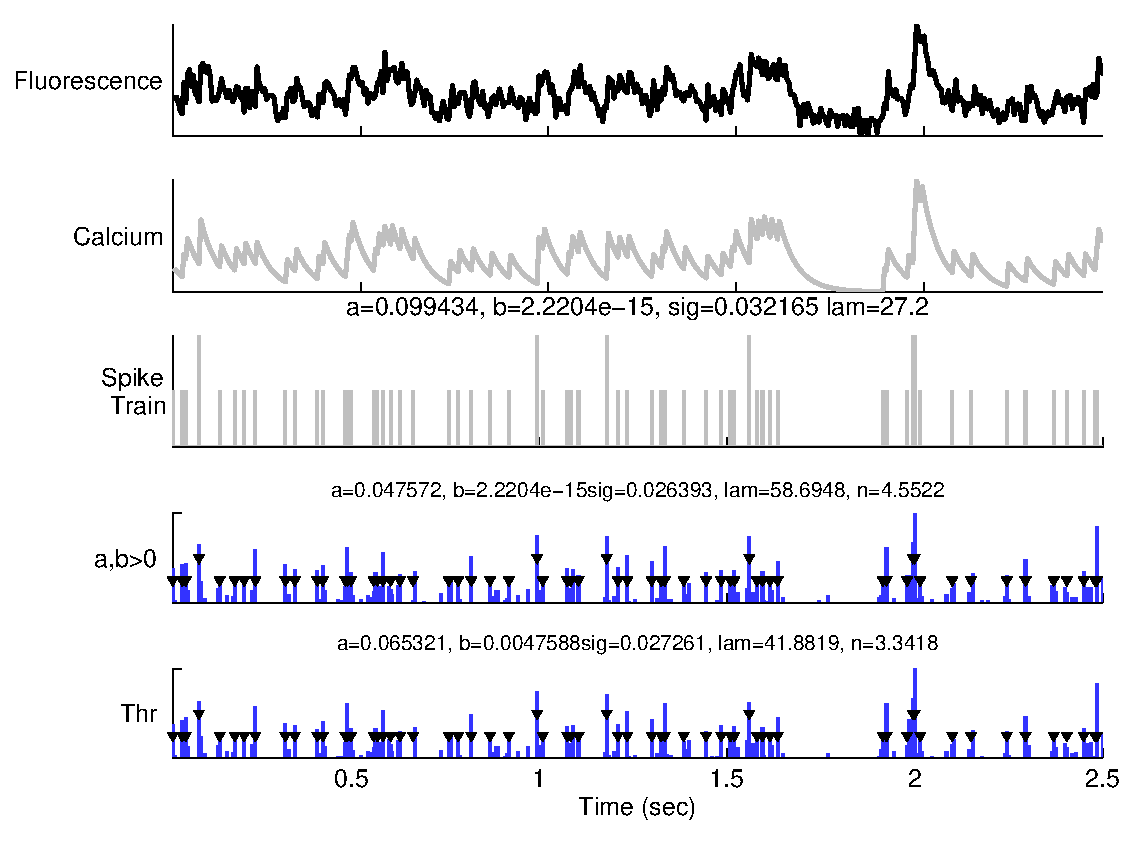
\includegraphics[width=.9\linewidth]{schem}
\caption{full movie, fully automated, real data} \label{fig:spatial_full_data}
\end{figure}




\subsection{Poisson observation model}

\subsection{Time varying prior}

\subsection{Slow dynamics}

\subsection{Incorporating a nonlinear observation model}

\subsection{Optimal thresholding}

\newpage
\section{Discussion}
We show here that for certain nonnegative deconvolution problems, we can derive an algorithm that is both optimal and efficient.  More specifically, our algorithm may be applied to any model with a nonnegative signal that is linearly filtered by a matrix linear ordinary differential equation.  We apply this approach to the problem of inferring the most likely spike train given noisy calcium sensitive fluorescence observations (c.f. Fig.\ \ref{fig:demo}), and demonstrate, in simulations, that the optimal nonnegative filter outperforms the optimal linear (i.e., Wiener) filter in both slow and fast firing rate regimes (c.f. Fig.\ \ref{fig:comp}).  Furthermore, when applied to data from a live cell, the optimal nonnegative filter outperforms a fast projection pursuit regression filter, which constrains the inferred spike train to be nonnegative integers (c.f. Fig.\ \ref{fig:real}). On the other hand, the nonnegative filter is based on a linear observation model, and therefore suffers a loss of precision in the presence of strong saturation effects, in contrast to the optimal nonlinear particle filter (c.f. Fig.\ \ref{fig:real}).    

The implications of these results are severalfold.  First, it seems as if there is no reason to use the Wiener filter for scenarios in which our algorithm may apply.  Second, as our filter is so efficient, it may be used for many real-time processing applications.  Specifically, upon simultaneously imaging a population of neurons \cite{IkegayaYuste04, NiellSmith05, OhkiReid05, YaksiFriedrich06, SatoSvoboda07}, our filter may be applied essentially online.  This could greatly expedite the tuning of important experimental parameters --- such as laser intensity --- to optimize signal-to-noise ratio for inferring spikes.  Third, the parameters estimated from this filter may be used to initialize the parameters of the optimal nonlinear particle filter, which may then be used offline, to further refine the spike train inference. % Because the optimal nonlinear particle filter performs in approximately real-time (making it $\sim 100$ fold slower than the filters developed here), it may be run overnight on all the neural data collected in a daily experimental session. 
%Future work will consider multidimensional models for this application, incorporating both more sophisticated calcium models, and spatial filtering for extracting the fluorescence signal, obviating the need for additional algorithms for image segmentation. 



\paragraph{Acknowledgments}

Support for JTV was provided by NIDCD DC00109. LP is supported by an NSF CAREER award, by an Alfred P.\ Sloan Research Fellowship, and the McKnight Scholar Award. BOW was supported by NDS grant F30 NS051964. The authors would like to thank A.\ Packer for helpful discussions.

%\subparagraph*{References}
\bibliography{/Users/joshyv/Research/misc/biblist}
\addcontentsline{toc}{section}{References}
%\bibliography{Science}
\bibliographystyle{apalike}
%\bibliographystyle{biophysj}
%\bibliographystyle{nature}


\appendix
\section{Wiener Filter}

Sections \ref{sec:inf} and \ref{sec:est} outline one approach to solving Eq. \eqref{eq:obj}, by approximating the Poisson distribution with an exponential distribution, and imposing a non-negative constraint on the inferred $\hnm$.  Perhaps a more straightforward approach would be to approximate the Poission distribution with a Gaussian distribution.  In fact, as rate increases above about $10$ spikes/sec, a Poisson distribution with rate $\lam \Del$ is well approximated by a Gaussian with mean and variance $\lam \Del$.  Given such an approximation, instead of Eq. \eqref{eq:obj2}, we would obtain:

\begin{align} \label{eq:w1}
\hbn_{w} &\approx \argmin_{n_t \in \Real, \forall t} \sum_{t=1}^T \bigg(\frac{1}{2\sig^2} (F_t-C_t)^2 + \frac{1}{2 \lam \Del} (n_t - \lam \Del)^2\bigg)% \nonumber \\
\end{align}

\noindent As above, we can rewrite Eq. \eqref{eq:w1} in matrix notation in terms of $\bC$:

\begin{align}   \label{eq:w2}
\hbC_{w}&= \argmin_{C_t \in \Real, \forall t} \frac{1}{2\sig^2} \norm{\bF - \bC}^2 + \frac{1}{2\lam\Del} \norm{\bM \bC - \lam\Del\ve{1}}^2 
\end{align}

\noindent which is quadratic in $\bC$, and may therefore be solved analytically using quadratic programming, $\hbC_w = \hbC_0 + \bd_w$, where $\hbC_0$ is the initial guess and $\bd_w=\bH_w \backslash \bg_w$, where

\begin{align}
\bg_w &= \frac{1}{\sig^2} (\bC_0' - \bF) + \frac{1}{\lam\Del} ( (\bM \hbC_0)' \bM - \lam\Del \bM' \ve{1}) \\
\bH_w &= \frac{1}{\sig^2} \ve{I} + \frac{1}{\lam\Del} \bM' \bM
\end{align}

Note that this solution is the optimal linear solution, under the assumption that spikes follow a Gaussian distribution, and if often referred to as the Wiener filter, regression with a smoothing prior, or ridge regression.  To estimate the parameters for the Wiener filter, we take the same approach as above:

\begin{subequations}
\begin{align} \label{eq:w_par}
\hbth_w &\approx \argmax_{\bth_w}P(\ve{F}| \hbn_w, \thet_w) P(\hbn_w | \thet_w) \\
%&= \argmax_{\bth_w} \sum_{t=1}^T \left(-\frac{1}{2} \log (2\pi\sig^2)-\frac{1}{2\sig^2} (F_t - \gamma \hC_{t-1} - \hn_t - \beta)^2 \right) \nonumber \\
%&\qquad \qquad \qquad + \sum_{t=1}^T \bigg(-\frac{1}{2} \log (2\pi\lam\Del)-\frac{1}{2\lam\Del} (\hn_t - \lam\Del)^2 \bigg) \\
&= \argmax_{\bth_w} -\frac{T}{2} \log (4\pi^2\sig^2\lam\Del) - \frac{1}{2\sig^2} \norm{\bY_w + \ve{\eta}_w \bX_w}^2 - \frac{1}{2\lam\Del} \norm{\hbn_w - \lam\Del\ve{1}}^2
\end{align}
\end{subequations}

\noindent where $\bY_w$, $\ve{\eta}_w$, and $\bX_w$ are defined as their subscriptless counterparts in Eq. \eqref{eq:par1}.




%\section{old}
%
%%\begin{algorithm}
%%\caption{Pseudocode for implementing the optimal nonnegative filter for an exponential prior} \label{alg:bar}
%%\begin{algorithmic}
%%\WHILE{$\zzz > \epsilon$}
%%\STATE Initialize $\zT$
%%\STATE $\mathcal{L}_i= \sum_t (\ve{y}_t - \ve{A} \ve{C}_t - \ve{b}) \ve{I}^{-1}  (\ve{y}_t - \ve{A} \ve{C}_t - \ve{b}) +\Del \lam_t n_t - \zzz \log n_t$
%%\WHILE{$\mathcal{L}_i < \mathcal{L}_{i-1}$}
%%\STATE $\ve{g} = -2  (\ve{y} - \ve{A} \xT - \ve{b}) - \Del \lT' \ve{M} - \zzz \ve{M}' (\zT^{-1})$
%%\STATE $\ma{H}= 2 \ve{I} + 2 \zzz \ve{M}' (\zT^{-2}) \ve{M}$
%%\STATE Compute $\ve{d}=\ma{H}^{-1}\ve{g}$ efficiently
%%\STATE Choose $s$ such that 
%%\STATE $\qquad s \geq -\zT(\ve{M} \ve{d})^{-1}$
%%\STATE $\qquad$and $\mathcal{L}_{i} < \mathcal{L}_{i-1}$
%%\STATE Let $\xT \leftarrow  \xT + s \ve{d}$
%%\STATE $i \leftarrow i + 1$
%%\ENDWHILE
%%\STATE reduce $\zzz$ 
%%\ENDWHILE
%%\end{algorithmic}
%%\end{algorithm}
%
%\newpage \begin{figure}
%%\centering 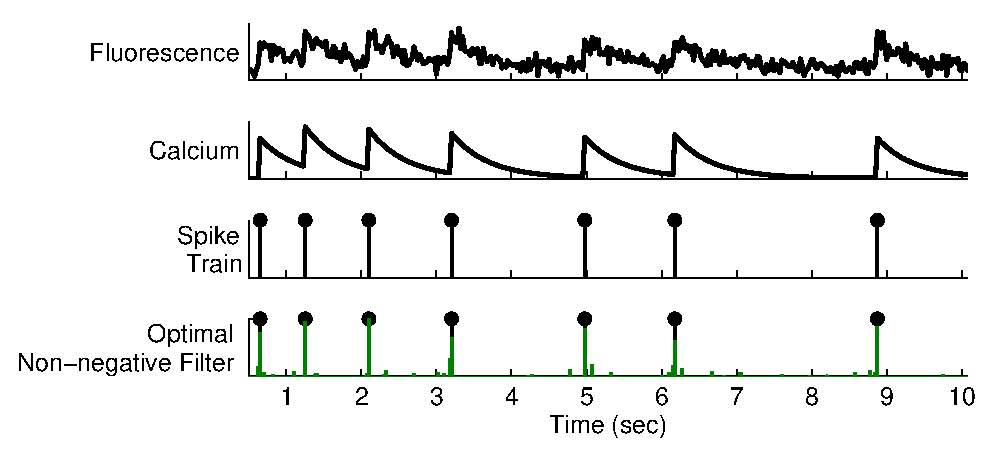
\includegraphics[width=0.7\linewidth]{NIPSdemo}
%\caption{Simulation demonstrating our neuron model and inference. Note that our filter accurately infers the unobserved spike train, given only the noisy fluorescence measurements.  Top panel: Simulated fluorescence. Second panel: Simulated intracellular calcium concentration. Third panel: Simulated spike train.  Fourth panel: Output of optimal nonnegative filter (green) superimposed on simulated spike train (black).  Parameters: $\lam=10$, $\Del=0.025$ msec, $\tau=0.5$ sec, $\sig=1$.} \label{fig:demo}
%\end{figure}
%
%\paragraph{Generalization of the optimal nonnegative filter}
%
%The above filter design assumed a very simple model relating spikes to $\Ca$, and $\Ca$ to fluorescence.  Both \eqref{eq:obs} and \eqref{eq:trans} may be generalized in a straightforward manner. In fact, our model may be thought of as a special case of the more general state-space framework:
%
%\begin{subequations} \label{eq:SS}
%\begin{align}
%\ve{C}_t &= \ve{D} \ve{C}_{t-1} + \ve{1} n_t \label{eq:SSa} \\
%\ve{F}_t &= \ve{A} \ve{C}_t + \ve{b} + \ve{\varepsilon}_t \label{eq:SSb}
%\end{align}
%\end{subequations}
%
%\noindent which we can solve in linear time for any log-concave distribution of $n_t$ and $\ve{\varepsilon}_t$.  For our particular scenario of interest, i.e., that of inferring spike trains from calcium sensitive fluorescence observations, these generalizations facilitate considering a model with much richer dynamics.  For instance, a more accurate model relating spikes to $\Ca$ would consider myriad calcium extrusion mechanisms, buffering, etc. In such a situation, we would represent $\Ca$ as a vector, $\ve{C}_t \in \mathbb{R}^{N \times 1}$, where each element of $\ve{C}_t$ would correspond 
%%
%%These may all easily be incorporated by replacing the monodimensional $\Ca$ equation, with %:
%%
%%\begin{align} \label{eq:C}
%%$\ve{C}_{t+1} = \ma{D} \ve{C}_t + \ve{1} n_t$ %, \qquad \ve{C}_t \geq 0 \quad \forall t
%%\end{align}
%%
%%\noindent 
%%where each element of $\ve{C}_t \in \mathbb{R}^{N \times 1}$ corresponds 
%to a different spike dependent calcium process. The differential operator, $\ve{D} \in \mathbb{R}^{N \times N}$, accounts for the relative strength of each of these mechanisms, and their time constants. The spikes, $n_t$, are multiplied by a column vector of ones, $\ve{1} \in \mathbb{R}^{N \times 1}$, because the magnitude of the effect of a spike on each element in $\ve{C}_t$ is scaled by $\ve{\rho}$.\footnote{For the same reasons that there is no parameter scaling the spikes in the monodimensional case} It should be clear that as in \eqref{eq:trans}, spikes are related to calcium by a simple linear transformation.  In the multidimensional scenario, however, $\ve{D}$ --- a matrix --- would replace $a$ --- a scalar ---  so $\ve{M}$ becomes block-bidiagonal, making the Hessian block tridiagonal.  Nonetheless, Gaussian elimination may still solve $\ve{H}\ve{C}=\ve{g}$ in $O(T)$, so our filter may be applied to this scenario as well.
%
%Another natural extension of this work would be to let $F_t$ also be multidimensional.  In \eqref{eq:obs}, although we assumed that we had access to a monodimensional fluorescent magnitude at each time, the raw data is actually a multidimensional movie. These images, however, are necessarily blurred by the point-spread-function of the camera.  Thus, we could replace \eqref{eq:obs} with \eqref{eq:SSb}, where $\ve{A}$ is the point-spread function of the camera, and $\ve{b}$ sets the relative baseline intensity per pixel. %\footnote{In practice, we would concatenate the columns of each image,  making $\ve{F}_t$ a column vector, $\ve{F}_t \in \mathbb{R}^{Q \times 1}$. Furthermore, $\ve{A} \in \mathbb{R}^{Q \times N}$, $\ve{A}$ would be a rank-one matrix, $\ve{A}=\ve{a} \ve{1}'$, where each element of $\ve{a}$ corresponds to the relative weight of each pixel. By parameterizing $\ve{a}$, we could limit the number of parameters for this multidimensional model to be relatively few.} 
%Furthermore, the noise, $\ve{\varepsilon}_t$, could have any log-concave distribution, and these results would still hold. Given these generalizations, this filter may be applied to a large class of problems.
%
%%nonnegative deconvolution \cite{SaulLee03} and matrix factorization \cite{LeeSeung99, LeeSeung01} arise in a number of different scenarios, including from audio signals processing \cite{OGradyPearlmutter06} and image processing. We are interested in dealing with a subset of these problems.
%%In particular, we assume the existence of a signal of interest, $\zT=n_0,\ldots,n_T$, where each $n_t \in \mathbb{R}_+$ is a scalar nonnegative number,  which is then filtered by a series of linear ordinary differential equations, of the form:
%%
%%\begin{align} \label{eq:C}
%%\ve{C}_{t+1} = \ma{a} (\ve{C}_t + \ve{C}_b) + \ve{1}  n_t %, \qquad \ve{C}_t \geq 0 \quad \forall t
%%\end{align}
%%
%%\noindent where $\ve{C}_t \in \mathbb{R}^{N \times 1}$ is an $N$ dimensional column vector, $\ma{a} \in \mathbb{R}^{N\times N}$ is a differential operator matrix that updates $\ve{C}_t$, $\ve{C}_b$ is the baseline resting value for $\ve{C}_t$, and $\ve{1}$ is a $N$ dimensional column vector of ones.  Observations of this system, $\ve{y}_t \in \mathbb{R}^{M \times 1}$,  are linear-Gaussian functions of $\ve{C}_t$:
%%
%%\begin{align} \label{eq:y}
%%\ve{y}_t = \ve{A} \ve{C}_t + \ve{b} + \ve{\varepsilon}_t, \qquad \ve{\varepsilon}_t \sim \mathcal{N}(0,\ve{I})
%%\end{align} 
%%
%%\noindent where $\ma{A} \in \mathbb{R}^{M\times N}$ is a scaling matrix,  $\ve{b} \in \mathbb{R}^{M \times 1}$ is an offset vector, and  $\varepsilon_t \in \mathbb{R}^{M \times 1}$ is a standard multivariate normal random variable.  Models characterized by \eqref{eq:trans} and \eqref{eq:y} arise in a number of contexts, including several in neuroscience \cite{bj08}.   
%%%This signal is then convoled with $J$ exponential filters, each with a unique amplitude and time constant, $A_j$ and $\tau_j$, respectively.  Finally, we make observations, $y_t$ that are corrupted by some Gaussian noise source, $\varepsilon_t$, with mean $\mu$ and variance $\sig^2$, yielding
%%%
%%%\begin{align}
%%%y_t = \sum_{j=1}^J \sum_{t=0}^T C_t \ast A_j e^{-t/\tau_j} + \varepsilon_t, \qquad \varepsilon \sim \mathcal{N}(\mu,\sig^2)
%%%\end{align}
%
%\paragraph{Projection Pursuit Regression} 
%
%Projection pursuit regression (PPR) is another technique one could use to infer a spike train from fluorescence measurements.  PPR is different from the optimal nonnegative filter in a few ways.  First, it solves a related, but slightly different problem: instead of finding the MAP estimate of the spike train, PPR finds the maximum likelihood estimate, i.e., the spike train that makes the fluorescence measurements most likely.  Second, PPR constrains the solution to have only nonnegative integers. Therefore, $\zT_{PPR}=\argmax_{n_t \in \mathbb{N}_0} p(\FT | \zT)$, where $\mathbb{N}_0$ is the set of nonnegative integers.. 
%% is the solution to the following optimization problem:
%%
%%\begin{align} \label{eq:ppr}
%%\nT_{PPR} = \argmax_{n_t \in \mathbb{n}} p(\FT | \nT)
%%\end{align} 
%%
%Third, because of this constraint, PPR requires an additional parameter, $w$, that sets the size of the calcium transient caused by a single an action potential.  This forces us to substitute \eqref{eq:trans}  with $C_t = a C_{t-1} + w n_t$.  % It may be helpful to think of $\CaT$ as a sum of exponentials, each starting at the time of an action potential.  
%%
%%More specifically, for this problem, PPR assumes that the signal of interest, $\FT$, is a sum of exponentials times Heaviside step functions and Gaussian noise:
%%
%%\begin{align}
%%\FT = \sum_{t_i} \rho e^{(t_i-t)/\tau} H(t_i-t) + \ve{\varepsilon}
%%\end{align}
%%
%%\noindent where $H(C)=1$ when $C\geq 0$ and zero otherwise, and the goal is to find the spike times, $\{t_i\}$. 
%Given these differences, to find $\zT_{PPR}$, PPR proceeds iteratively, adding a spike with each iteration, as long as doing so reduces the residual square error (i.e., the sum of the squared difference between the inferred $\xT$ and $\FT$). One obtains the time of the next inferred spike by finding the maximum of the convolution of the current residual square error with the calcium kernel, $w e^{-t\Del/\tau}$. In general, this procedure takes $O(T \log T)$ per iteration, as the convolution is computed in the Fourier domain.  However, the recursive state-space representation in \eqref{eq:SS} implies that this convolution requires just $O(T)$ time here.  Henceforth, we therefore refer to this approach as fast PPR (or fPPR). This approach may generalized to the multidimensional cases, as in the previous filter. However, unlike the previous filter, the likelihood function is not concave (recall that PPR is a greedy optimization method), so we are no longer guaranteed to converge to the optimal solution. % Nonetheless, this algorithm performs very well for simulated data, as depicted by the bottom panels of Fig. \ref{fig:comp}. 
%%Learning the parameters for this model proceeds much like learning those for the optimal nonnegative filter. 
%
%\section{Results} \label{sec:results} %Comparison to other methods}\label{sec:comp}
%
%To evaluate the efficacy of our filters, we compare their results to that of the optimal linear (i.e., Wiener) filter \cite{Wiener49}.  The Wiener filter differs in construction from our filters in a few ways.  First, it imposes no constraint on on the spike train.  Second, it is optimal upon assuming that the prior distribution of $n_t$ is Gaussian. In our model, spiking was Poisson, \eqref{eq:trans}, and the nonnegativity of $n_t$ in the sparse-spiking regime makes the Gaussian model assumed by the Wiener filter inaccurate (Fig.\ 2, left).  However, when spike rates are fast --- e.g., on average, several spikes per image frame --- a Poisson distribution is better approximated by a Gaussian distribution.  Furthermore, at high firing rates, the mean of the Gaussian would be relatively far from zero, and the variance proportional, so the probability of sampling a negative number would be relatively small, obviating the need for the nonnegativity constraint. Thus, one might expect the Wiener filter to perform as well as our nonnegative filter (and fPPR) when the observed neuron has a high firing rate (and relatively low imaging rate). Furthermore, given that the calcium kernel is exponential, the Wiener filter, like the filters we developed here, only requires $O(T)$ time, as opposed to the typical $O(T\log T)$.
%
%Fig.\ \ref{fig:comp} depicts a comparison between the filters developed above and the Wiener filter for two different scenarios: a slow firing rate simulation (left panels) and a fast firing rate simulation (right panels). When action potentials are sparse, the two filters we propose above outperform the Wiener filter. Moreover, at high firing rates,  all three filters perform approximately equally well. 
%
%%Perhaps the most closely related filter to the filters developed above is the Wiener filter \cite{??}.   Fig. \ref{fig:comp} shows two example fluorescent traces.  One the left, a neuron was simulated with a rate of $1$ Hz; on the right, $10$ Hz. The top and second panels show the simulated fluorescence and spike train, respectively.  The third panels show the performance of the optimal linear (i.e., Wiener) filter; whereas the fourth panels show the performance of the optimal nonnegative filter. Both filters perform very well in the scenario when there are on average several spikes per frame.   
%
%%\begin{minipage}{1.0\textwidth}
%\newpage \begin{figure}
%%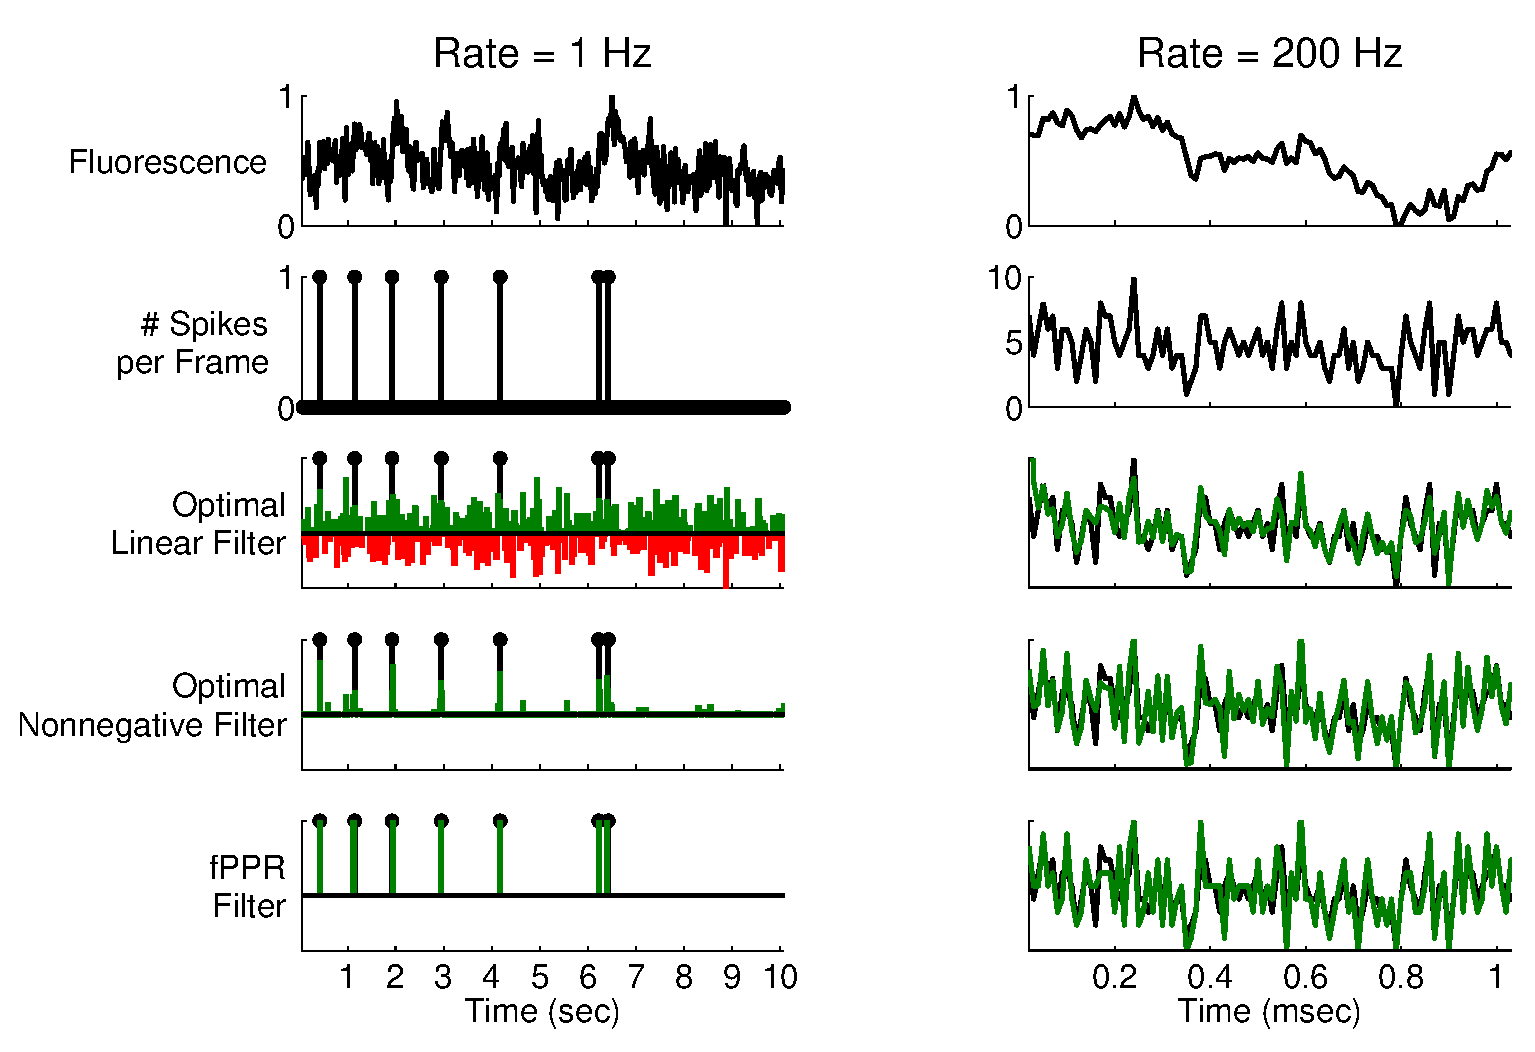
\includegraphics[width=1.0\linewidth]{NIPScomp}
%\caption{Comparison of various linear filters for a simulated Poisson neuron spiking with a rate of $1$ Hz (left panels) and $200$ Hz (right panels). The main result is that the two filters proposed outperform the optimal linear (i.e., Wiener) filter. Top panels: Fluorescence measurements.  Second panels: Number of spikes per frame.  Third panels: Optimal linear (i.e., Wiener) filter output given the above fluorescence signal.  The Wiener filter does not impose a nonnegativity constraint, thus the inferred spike train can either be positive (green) or negative (red).  Fourth panels: Same as third panels, but for the optimal nonnegative filter. Note the absence of negative spikes.  Fifth panels: Same as third panels, but using the fast Projection Pursuit Regression (fPPR) filter. Parameters: $\Del=0.025$ sec, $\tau=0.5$ sec, $\lam=1/($firing rate$)$, left  $\sig=0.4$, right $\sig=1$.} \label{fig:comp}
%\end{figure}
%
%\newpage \begin{figure}[!h]
%%\centering 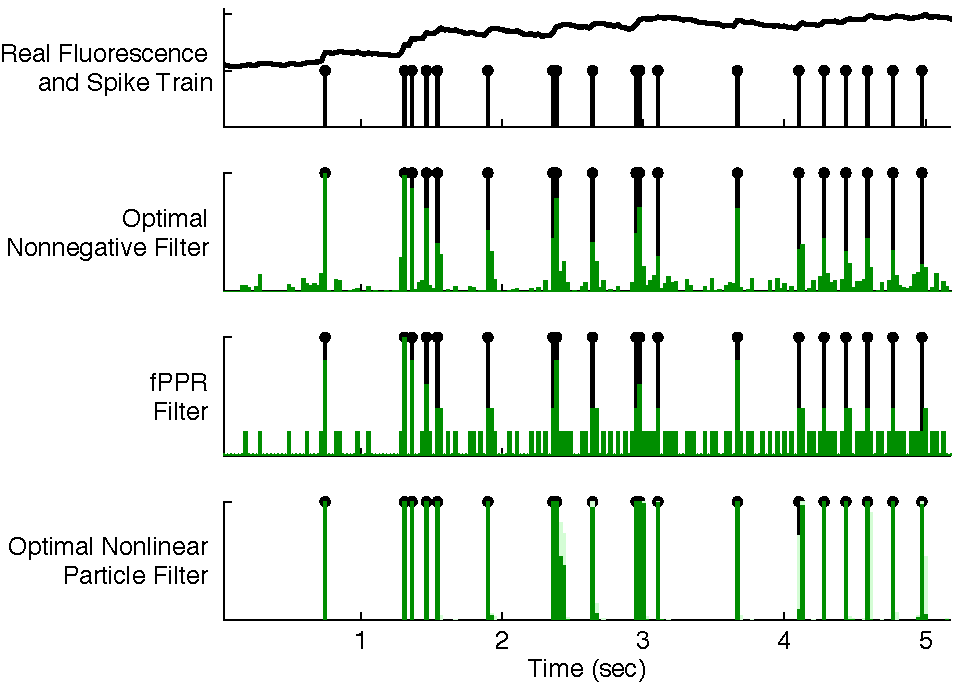
\includegraphics[width=.6\linewidth]{NIPSdata}
%\caption{Inferring a spike train given fluorescence measurements from a live \emph{in vitro} neuron.  Simultaneous recording of a saturating fluorescence signal (black line in top panel), and its associated spike train (black impluses in all panels).  Note how the three filters handle saturation differently. The optimal nonnegative filter's signal-to-noise ratio degrades as saturation increases, but does not suffer a catastrophic failure (green in second panel). fPPR suffers more than the optimal nonlinear particle filter when the signal saturates, due to the hard threshold (green in third panel). The optimal nonlinear particle filter \cite{BJ08}, which explicitly incorporates saturation, correctly identifies each spike time (green in bottom panel).} \label{fig:real}
%\end{figure}
%%\end{minipage}
%
%While in simulations, all the above algorithms perform reasonably well, the true test is how well they perform given data from live cells. We simultaneously recorded both electrophysiologically and imaged with an epifluorescent microscope, from a pyramidal neuron in a somatosensory cortical slice, as described in \cite{MacLeanYuste05}. Fig.\ \ref{fig:real} shows an example fluorescence time-series in which the neuron spiked with a relatively low rate, but the calcium accumulated nonetheless, leading to fluorescence saturation (top panel). In practice, this kind of strong saturation is rarely observed (personal communication, anonymous% R.\ Friedrich
%), so this example is designed to test the limits of performance of our filters. %As all the above described methods are inherently linear methods, their assumptions do not adequately capture these nonlinear dynamics.
%In fact, the optimal nonnegative filter accurately infers every spike, even when the fluorescence is strongly saturating, and the signal-to-noise ratio is very poor (second panel). On the other hand, fPPR, which has a sharp threshold for including an additional spike, performs relatively poorly (third panel), demonstrating the dependency of this method on a good model fit.  For comparison purposes, we also show the performance of an optimal nonlinear particle filter \cite{BJ08}, which specifically incorporates a nonlinear saturation function. While the optimal nonlinear particle filter performs better in scenarios such as this one, the computational burden is increased by approximately $100$-fold relative to the fast nonnegative filter. Thus these two filters serve complementary purposes: the fast nonnegative filter is better geared to rapid online analysis of large-scale multi-neuronal data, whereas the nonlinear particle filter is better suited for offline refinement of the results from the fast nonnegative filter.   
%
%z\section{Conclusions} \label{sec:dis}
%

%\section{other}
%
%We have found empirically that despite the approximation in \eqref{eq:obj2}, upon initializing the parameters with a reasonable guess, the algorithm tends to converge to parameters that are reasonably close to the true parameters, resulting in an accurate spike reconstruction. Importantly, estimating these parameters typically requires only a very short sequence of observations, e.g., several seconds of data including about $5$--$10$ spikes (not shown).
%


%\newpage \begin{figure}[H]
%%\centering 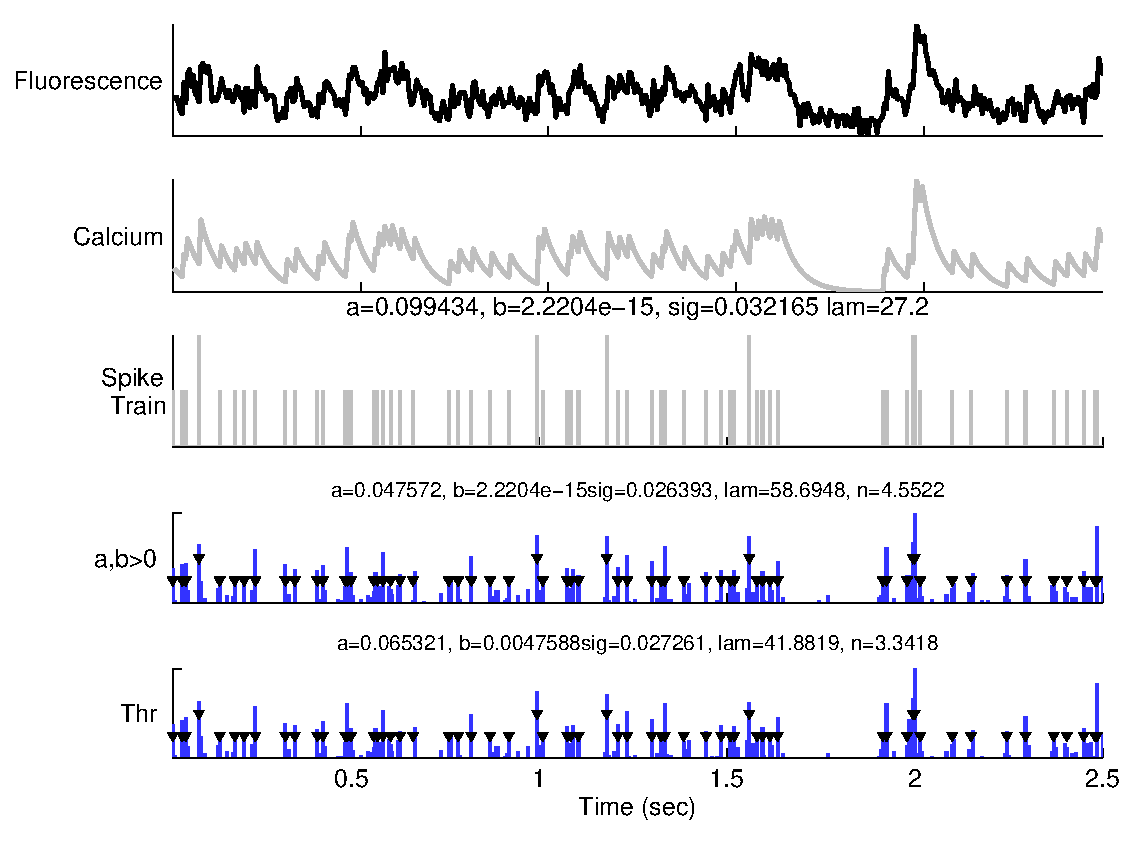
\includegraphics[width=.9\linewidth]{schem}
%\caption{same as spatial EM, but now have slow rise time on F} \label{fig:slow_rise}
%\end{figure}
%
%\newpage \begin{figure}[H]
%%\centering 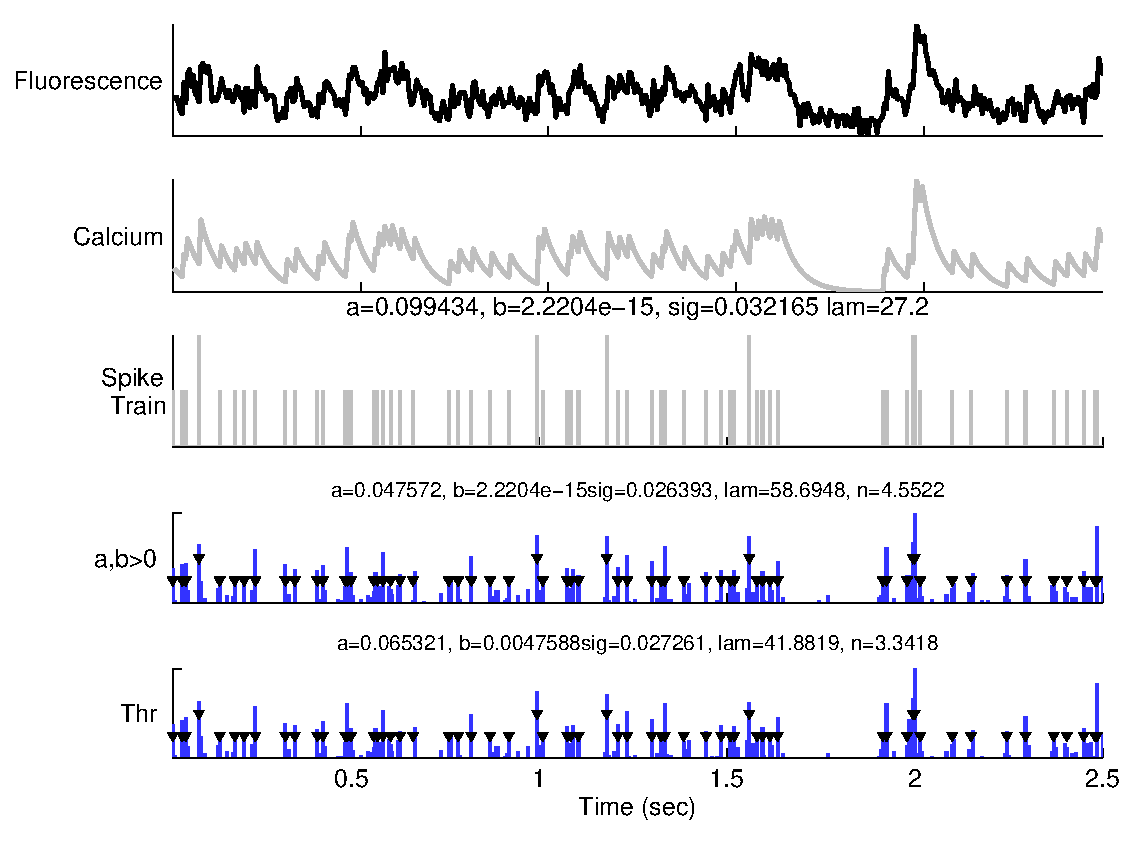
\includegraphics[width=.9\linewidth]{schem}
%\caption{same as spatial EM, but now have nonlinear observations} \label{fig:nonlin}
%\end{figure}
%
%\newpage \begin{figure}[H]
%%\centering 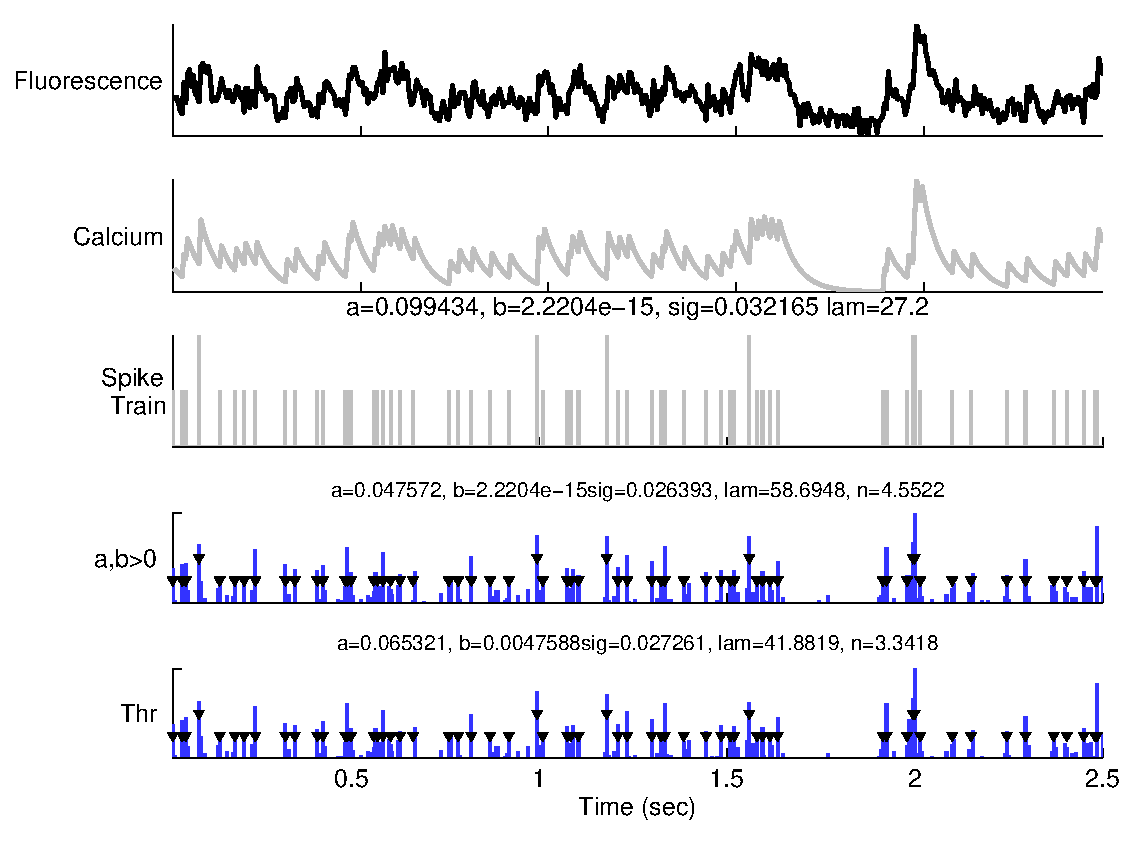
\includegraphics[width=.9\linewidth]{schem}
%\caption{same as spatial EM, but now have poisson observations} \label{fig:poisson}
%\end{figure}
%
%\newpage \begin{figure}[H]
%%\centering 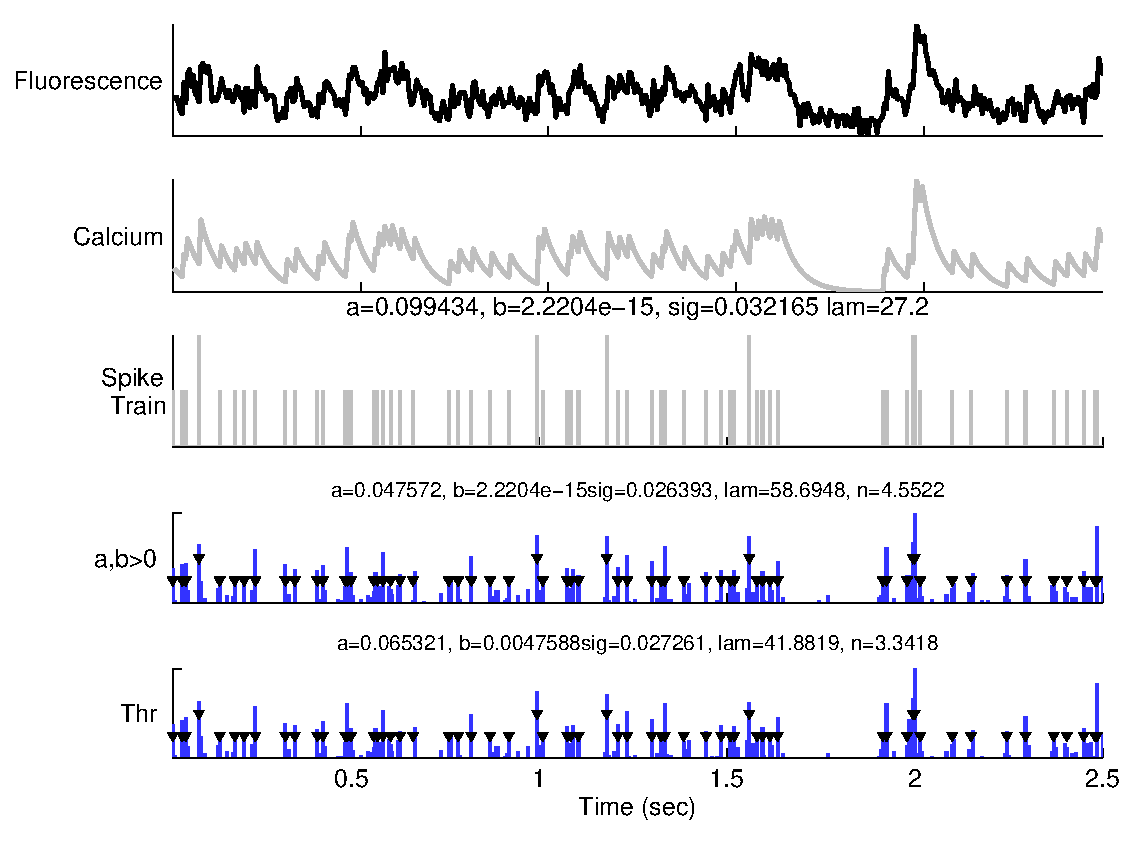
\includegraphics[width=.9\linewidth]{schem}
%\caption{drift}
%\end{figure}
%
%\newpage \begin{figure}[H]
%%\centering 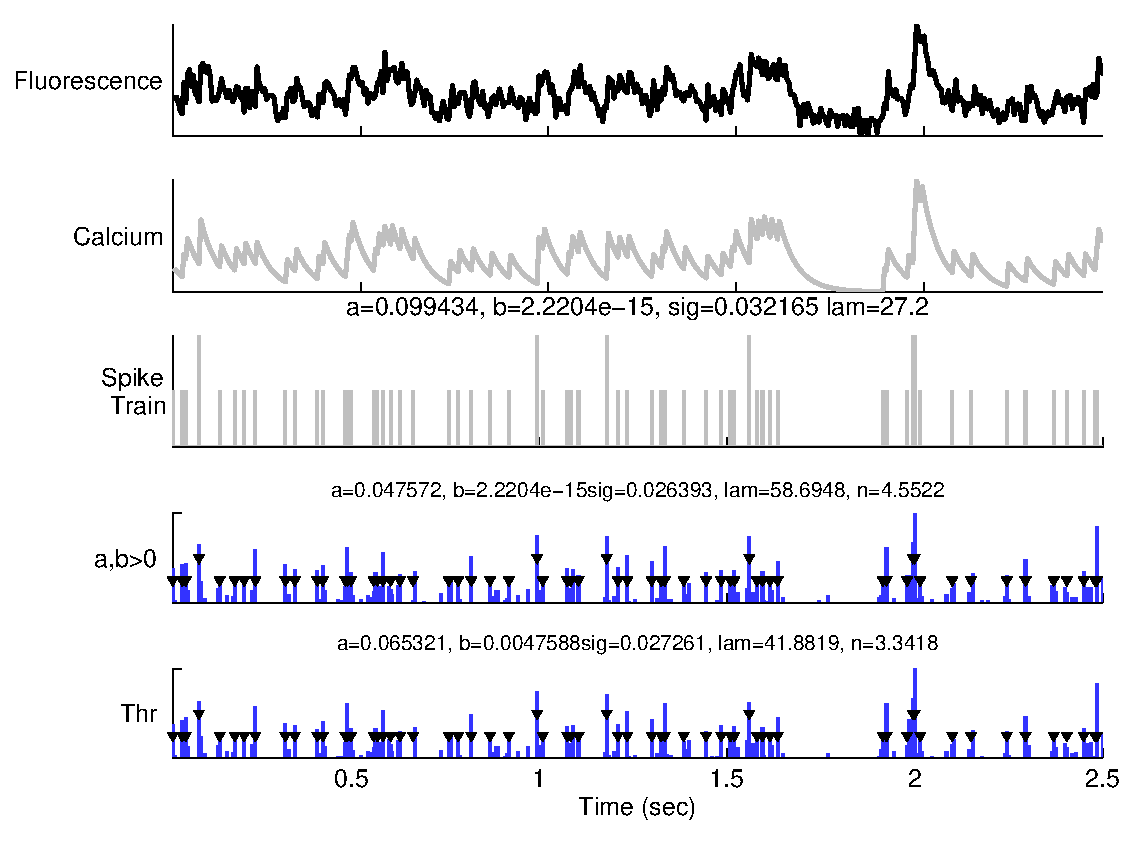
\includegraphics[width=.9\linewidth]{schem}
%\caption{thresholding}
%\end{figure}
%

\end{document}